\pdfminorversion=6 % this is needed to be able to include pdf 1.6. 
                    % For some reasons some old HPSG proceedings have pdf 1.6
\documentclass[11pt,a4paper,fleqn]{article}
\usepackage{times}
\thispagestyle{empty}



\usepackage[T1]{fontenc}   % Silbentrennung

\usepackage[utf8x]{inputenc}
                                                                                                                             
\hyphenation{Acad-e-my}

\usepackage[bookmarks=true,bookmarksopen=true,%
breaklinks=true,%
draft=false,plainpages=false,hyperfootnotes=false,%
pdfauthor={Stefan Müller (Editor)},%
pdftitle={Proceedings of the 15th International Conference on Head-Driven Phrase Structure Grammar},%
pdfkeywords={HPSG}%,
pdftex=true%
%ps2pdf=true  %ohne diesen Treiber geht der Zeilenumbruch in URLs
]{hyperref}% for pdf files
\hypersetup{colorlinks=false, pdfborder={0 0 0}}

\usepackage{pdfpages}
\pdfinclusioncopyfonts=1

\newcommand\formatauthor[2]{\begin{tabular}[t]{@{}c@{}}
  {\LARGE#1\strut}\\
  {\small#2\strut}\\
  \rule{\dimexpr0.5\linewidth-1em}{0pt}
  \end{tabular}\xhfill\ignorespaces}
\newcommand\xhfill{\hspace{1em plus 1fill}}

\begin{document}

\begin{center}
{\Large
                {\bfseries Proceedings of the 15th International Conference on\par Head-Driven Phrase Structure Grammar\par}

                \vspace{8ex}

                     National Institute of Information and Communications Technology, Keihanna\\[\baselineskip]

                        Stefan M{\"u}ller (Editor)\\[\baselineskip]

                                2008\\[\baselineskip]

                          CSLI Publications\\[\baselineskip]

              http://csli-publications.stanford.edu/HPSG/2008 \\[4\baselineskip]

The papers are published under a \href{http://creativecommons.org/licenses/by/4.0/}{CC-BY license}:\\[3pt]
\href{http://creativecommons.org/licenses/by/4.0/}{http://creativecommons.org/licenses/by/4.0/}
}
\end{center}
\newpage
\tableofcontents

\newpage

\section{Editor's Note}
%% -*- coding:utf-8 -*-
The 15th International Conference on Head-Driven Phrase Structure Grammar (2008) was held in Keihanna, Japan
and organized by the National Institute of Information and Communications Technology and the Shoin Institute for Linguistic Sciences,
Shoin Women's University.

The conference featured 2 invited talks and 17 papers
selected by the program committee 
(Anne Abeillé,
Olivier Bonami,
Francis Bond,
Bob Borsley,
Gosse Bouma,
Rui Chaves,
Berthold Crysmann,
Markus Egg,
Elisabet Engdahl,
Dan Flickinger,
Jonathan Ginzburg,
Danièle Godard,
Takao Gunji,
Chikara Hashimoto,
Erhard Hinrichs,
Anke Holler,
Chiharu Uda Kikuta,
Jong-Bok Kim,
Tibor Kiss,
Anna Kupsc,
Shalom Lappin,
Robert Levine,
Rob Malouf,
Nurit Melnik,
Detmar Meurers,
Stefan Müller,
Tsuneko Nakazawa,
Gerald Penn,
Adam Przepiórkowski,
Frank Richter,
Louisa Sadler,
Ivan Sag,
Manfred Sailer,
Jesse Tseng,
Stephen Wechsler,
Sh{\^{u}}ichi Yatabe (chair),
Kei Yoshimoto).

A workshop about \emph{Grammar at the Interfaces}
was attached to the conference. It featured one invited talk and 7 papers, selected by the program committee.

In total there were 34 submissions to the main conference and to the
workshop. 
We want to thank the respective program committee for putting this nice program together.



Thanks go to Francis Bond, Takao Gunji, Sanae Fujita, Kyoko Kanzaki, Taka\-yuki Kuribayashi, and Eric
Nichols, who were in charge of local arrangements.


As in the past years the contributions to the conference proceedings are based on the five page abstract
that was reviewed by the respective program committees, but there is no additional reviewing of the
longer contribution to the proceedings.
To ensure easy access and fast publication we have chosen an electronic format.


The proceedings include all the papers except those by Stefan Müller and Tsuneko Nakazawa.



\newpage
\part{Contributions to the Main Conference}
\thispagestyle{empty}
\newpage
        \setcounter{page}{6}
        \phantomsection
        \addcontentsline{toc}{section}{Emily M. Bender: Radical Non-Configurationality without Shuffle Operators: An Analysis of Wambaya}
\thispagestyle{empty}

\begin{center}
  {\huge\bfseries Radical Non-Configurationality without Shuffle Operators: An Analysis of Wambaya\par}

  \bigskip

~\\
\begingroup
\setlength{\leftskip}{0pt plus 1fill}
\setlength{\rightskip}{0pt plus 1fill}
\setlength{\parindent}{0pt}
\setlength{\parfillskip}{0pt}
  \formatauthor{Emily M. Bender}{\begin{tabular}{@{}c@{}}University of Washington\end{tabular}}

\par\endgroup

  \vspace*{8ex}

  Proceedings of the 15th International Conference on\par Head-Driven Phrase Structure Grammar

  \bigskip

  National Institute of Information and Communications Technology, Keihanna

  \medskip

  Stefan Müller (Editor)

  \medskip

  2008

  \medskip

  CSLI Publications

  \medskip

  pages 6--24

  \medskip

  \url{http://csli-publications.stanford.edu/HPSG/2008}
\end{center}
\vfill

\noindent



\vfill
\noindent
% APA Style
Bender, Emily M. 2008. Radical Non-Configurationality without Shuffle Operators: An Analysis of Wambaya. In Müller, Stefan (Ed.), \emph{{Proceedings of the 15th International Conference on Head-Driven Phrase Structure Grammar, National Institute of Information and Communications Technology, Keihanna}}, 6--24. Stanford,
CA: CSLI Publications. \hfill\href{http://creativecommons.org/licenses/by/4.0/}{\includegraphics[height=.75em]{Includes/ccby.eps}}

\newpage
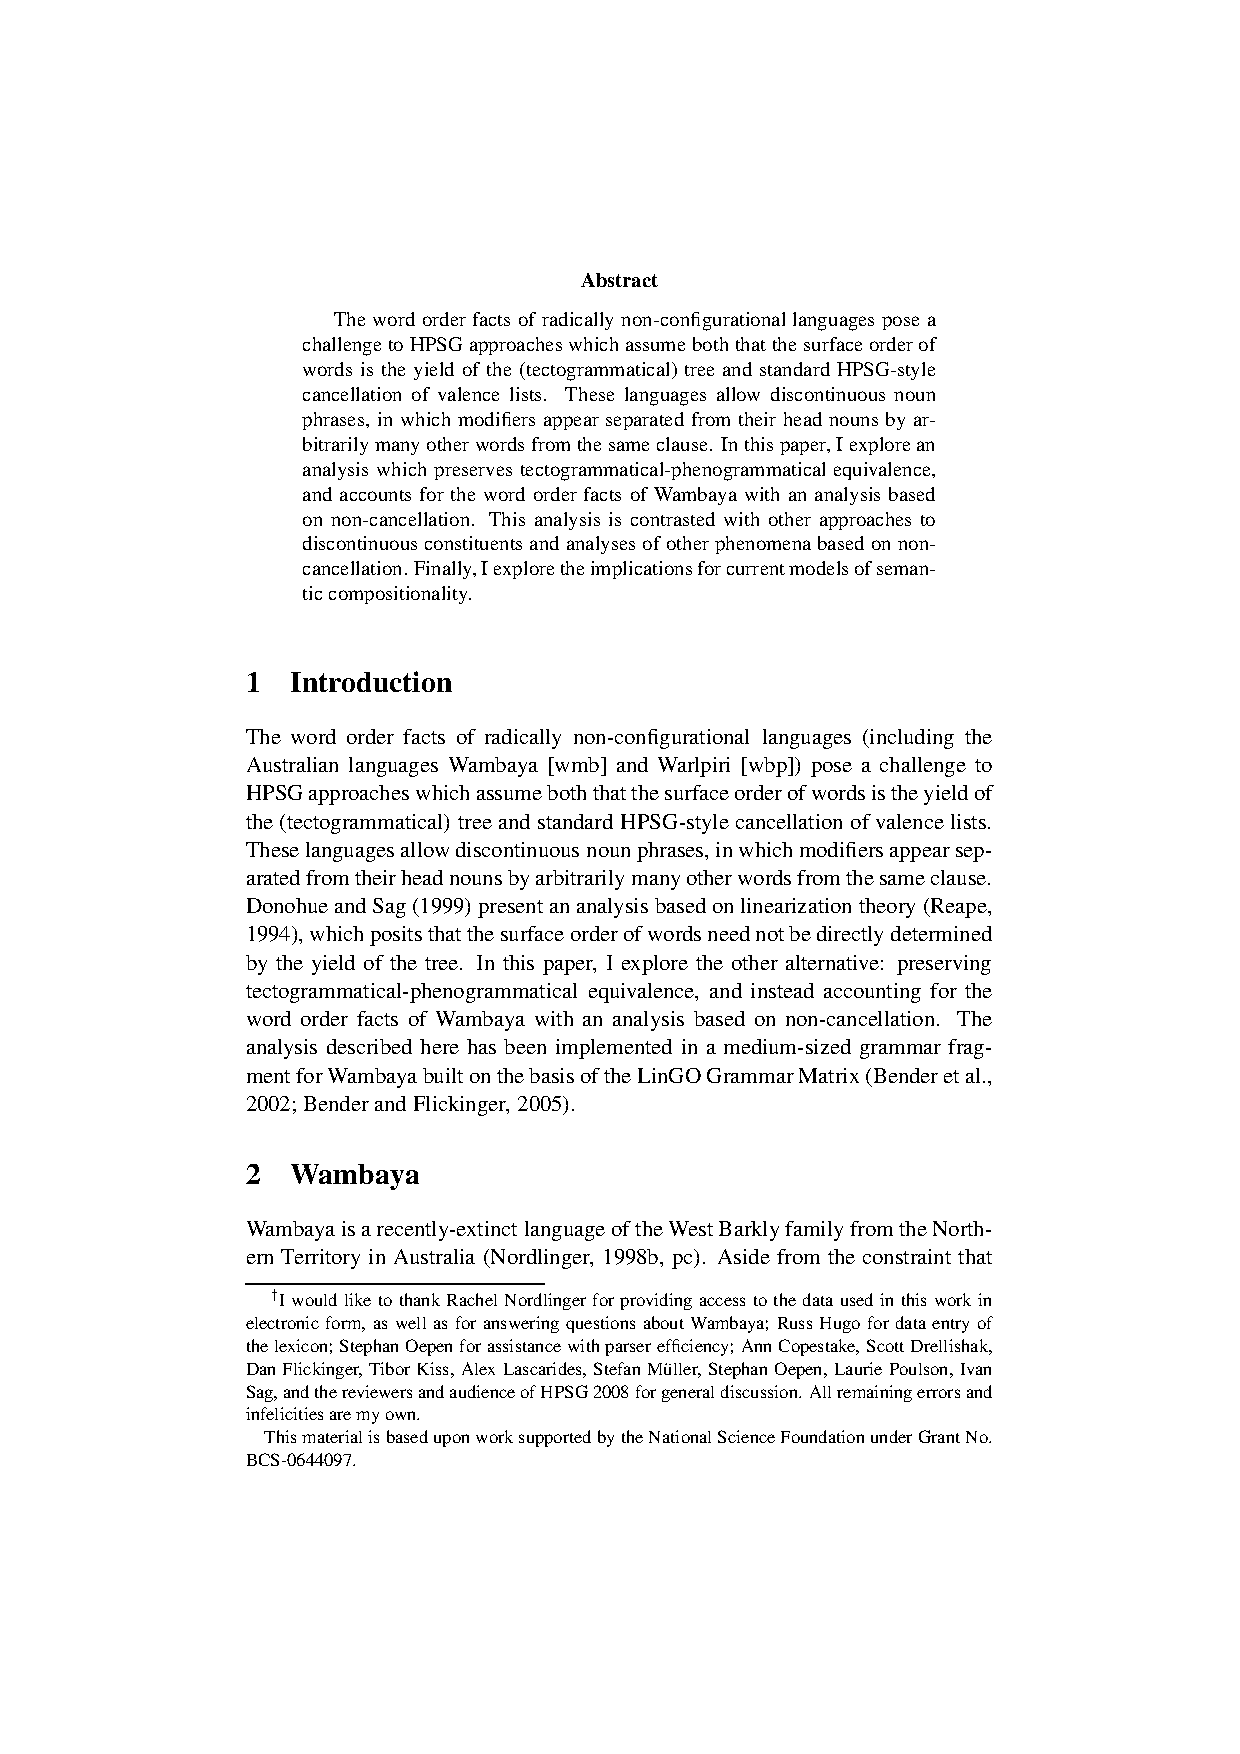
\includepdf[pages=-,pagecommand=\thispagestyle{plain}]{Includes/bender.pdf}
        \setcounter{page}{25}
        \phantomsection
        \addcontentsline{toc}{section}{Gabriela Bîlbîie: A Syntactic Account of Romanian Correlative Coordination from a Romance Perspective}
\thispagestyle{empty}

\begin{center}
  {\huge\bfseries A Syntactic Account of Romanian Correlative Coordination from a Romance Perspective\par}

  \bigskip

~\\
\begingroup
\setlength{\leftskip}{0pt plus 1fill}
\setlength{\rightskip}{0pt plus 1fill}
\setlength{\parindent}{0pt}
\setlength{\parfillskip}{0pt}
  \formatauthor{Gabriela Bîlbîie}{\begin{tabular}{@{}c@{}}University Paris 7\end{tabular}}

\par\endgroup

  \vspace*{8ex}

  Proceedings of the 15th International Conference on\par Head-Driven Phrase Structure Grammar

  \bigskip

  National Institute of Information and Communications Technology, Keihanna

  \medskip

  Stefan Müller (Editor)

  \medskip

  2008

  \medskip

  CSLI Publications

  \medskip

  pages 25--45

  \medskip

  \url{http://csli-publications.stanford.edu/HPSG/2008}
\end{center}
\vfill

\noindent



\vfill
\noindent
% APA Style
Bîlbîie, Gabriela. 2008. A Syntactic Account of Romanian Correlative Coordination from a Romance Perspective. In Müller, Stefan (Ed.), \emph{{Proceedings of the 15th International Conference on Head-Driven Phrase Structure Grammar, National Institute of Information and Communications Technology, Keihanna}}, 25--45. Stanford,
CA: CSLI Publications. \hfill\href{http://creativecommons.org/licenses/by/4.0/}{\includegraphics[height=.75em]{Includes/ccby.eps}}

\newpage
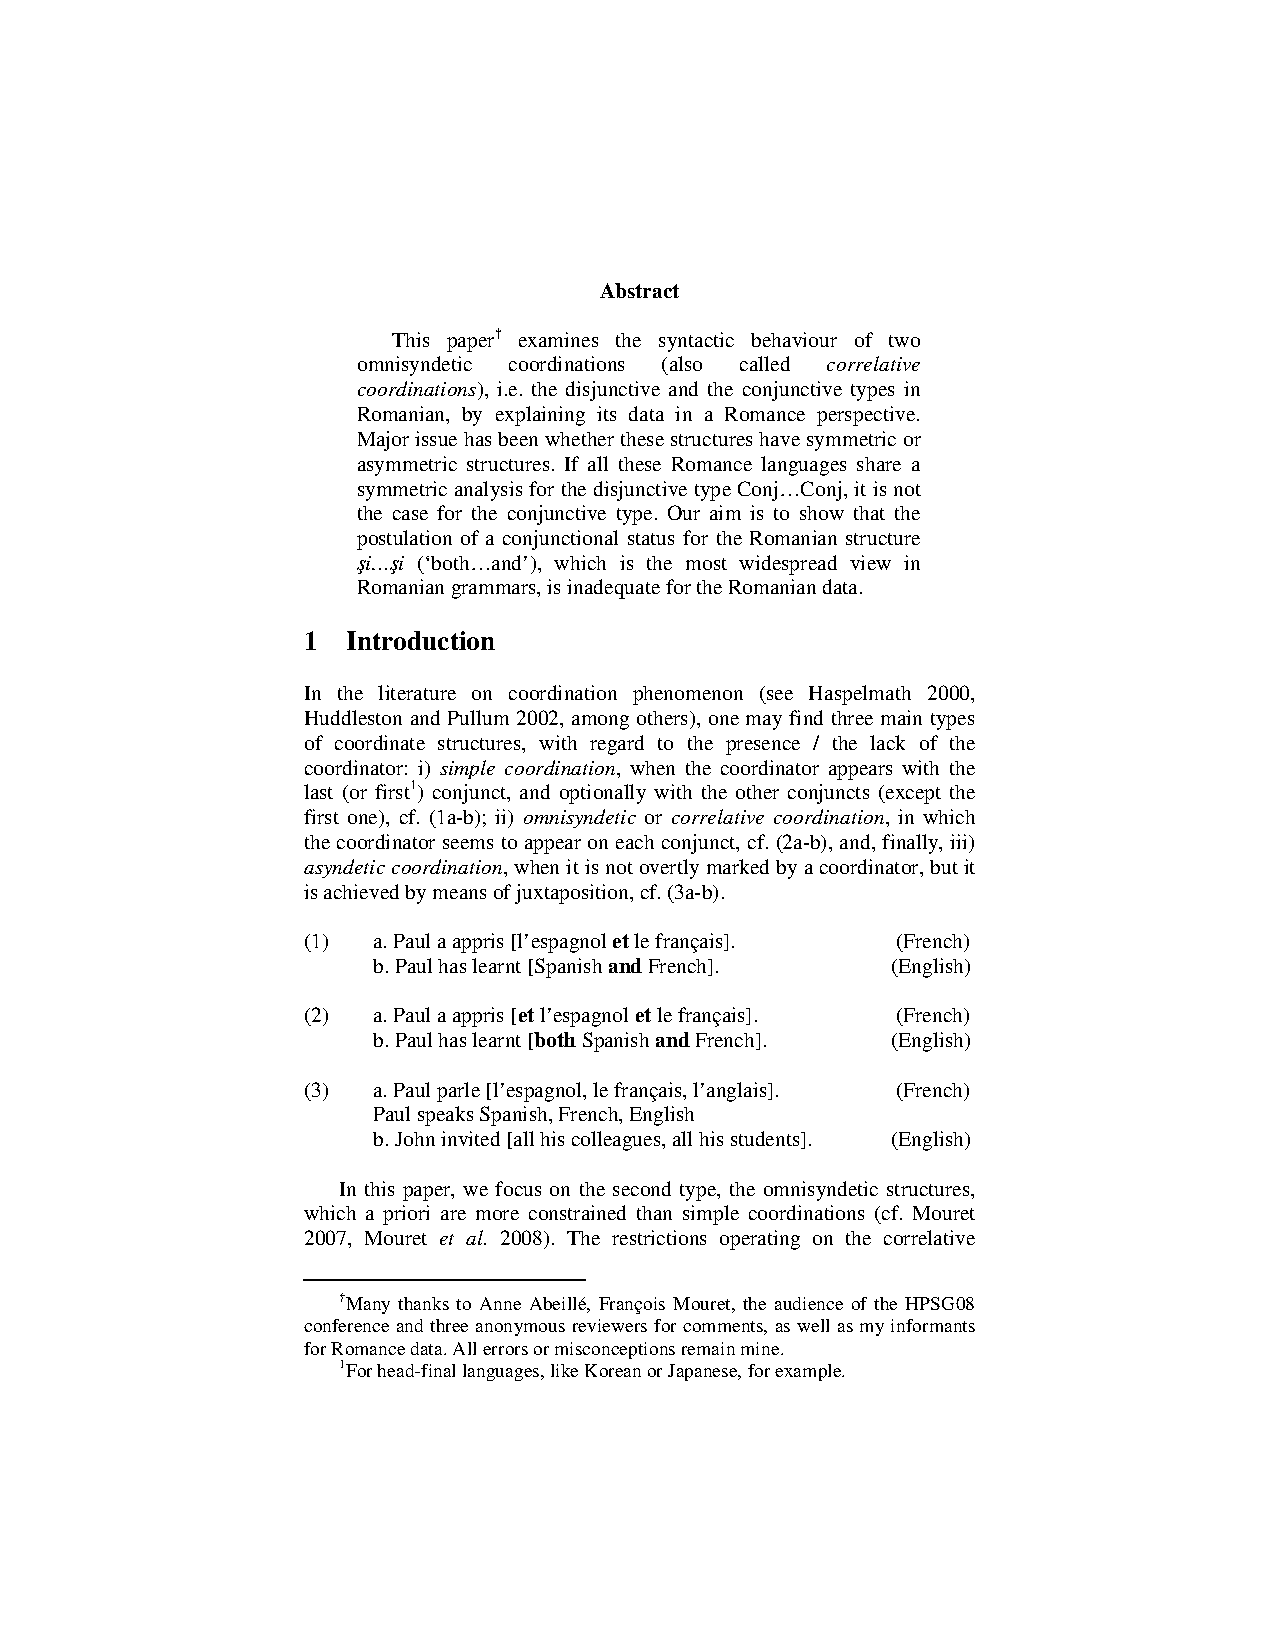
\includepdf[pages=-,pagecommand=\thispagestyle{plain}]{Includes/bilbiie.pdf}
        \setcounter{page}{46}
        \phantomsection
        \addcontentsline{toc}{section}{Anne Bjerre, Tavs Bjerre: \emph{There}-constructions with transitive verbs}
\thispagestyle{empty}

\begin{center}
  {\huge\bfseries \emph{There}-constructions with transitive verbs\par}

  \bigskip

~\\
\begingroup
\setlength{\leftskip}{0pt plus 1fill}
\setlength{\rightskip}{0pt plus 1fill}
\setlength{\parindent}{0pt}
\setlength{\parfillskip}{0pt}
  \formatauthor{Anne Bjerre}{\begin{tabular}{@{}c@{}}University of Southern Denmark\end{tabular}}
\formatauthor{Tavs Bjerre}{\begin{tabular}{@{}c@{}}Aarhus University\end{tabular}}

\par\endgroup

  \vspace*{8ex}

  Proceedings of the 15th International Conference on\par Head-Driven Phrase Structure Grammar

  \bigskip

  National Institute of Information and Communications Technology, Keihanna

  \medskip

  Stefan Müller (Editor)

  \medskip

  2008

  \medskip

  CSLI Publications

  \medskip

  pages 46--66

  \medskip

  \url{http://csli-publications.stanford.edu/HPSG/2008}
\end{center}
\vfill

\noindent



\vfill
\noindent
% APA Style
Bjerre, Anne, \& Bjerre, Tavs. 2008. \emph{There}-constructions with transitive verbs. In Müller, Stefan (Ed.), \emph{{Proceedings of the 15th International Conference on Head-Driven Phrase Structure Grammar, National Institute of Information and Communications Technology, Keihanna}}, 46--66. Stanford,
CA: CSLI Publications. \hfill\href{http://creativecommons.org/licenses/by/4.0/}{\includegraphics[height=.75em]{Includes/ccby.eps}}

\newpage
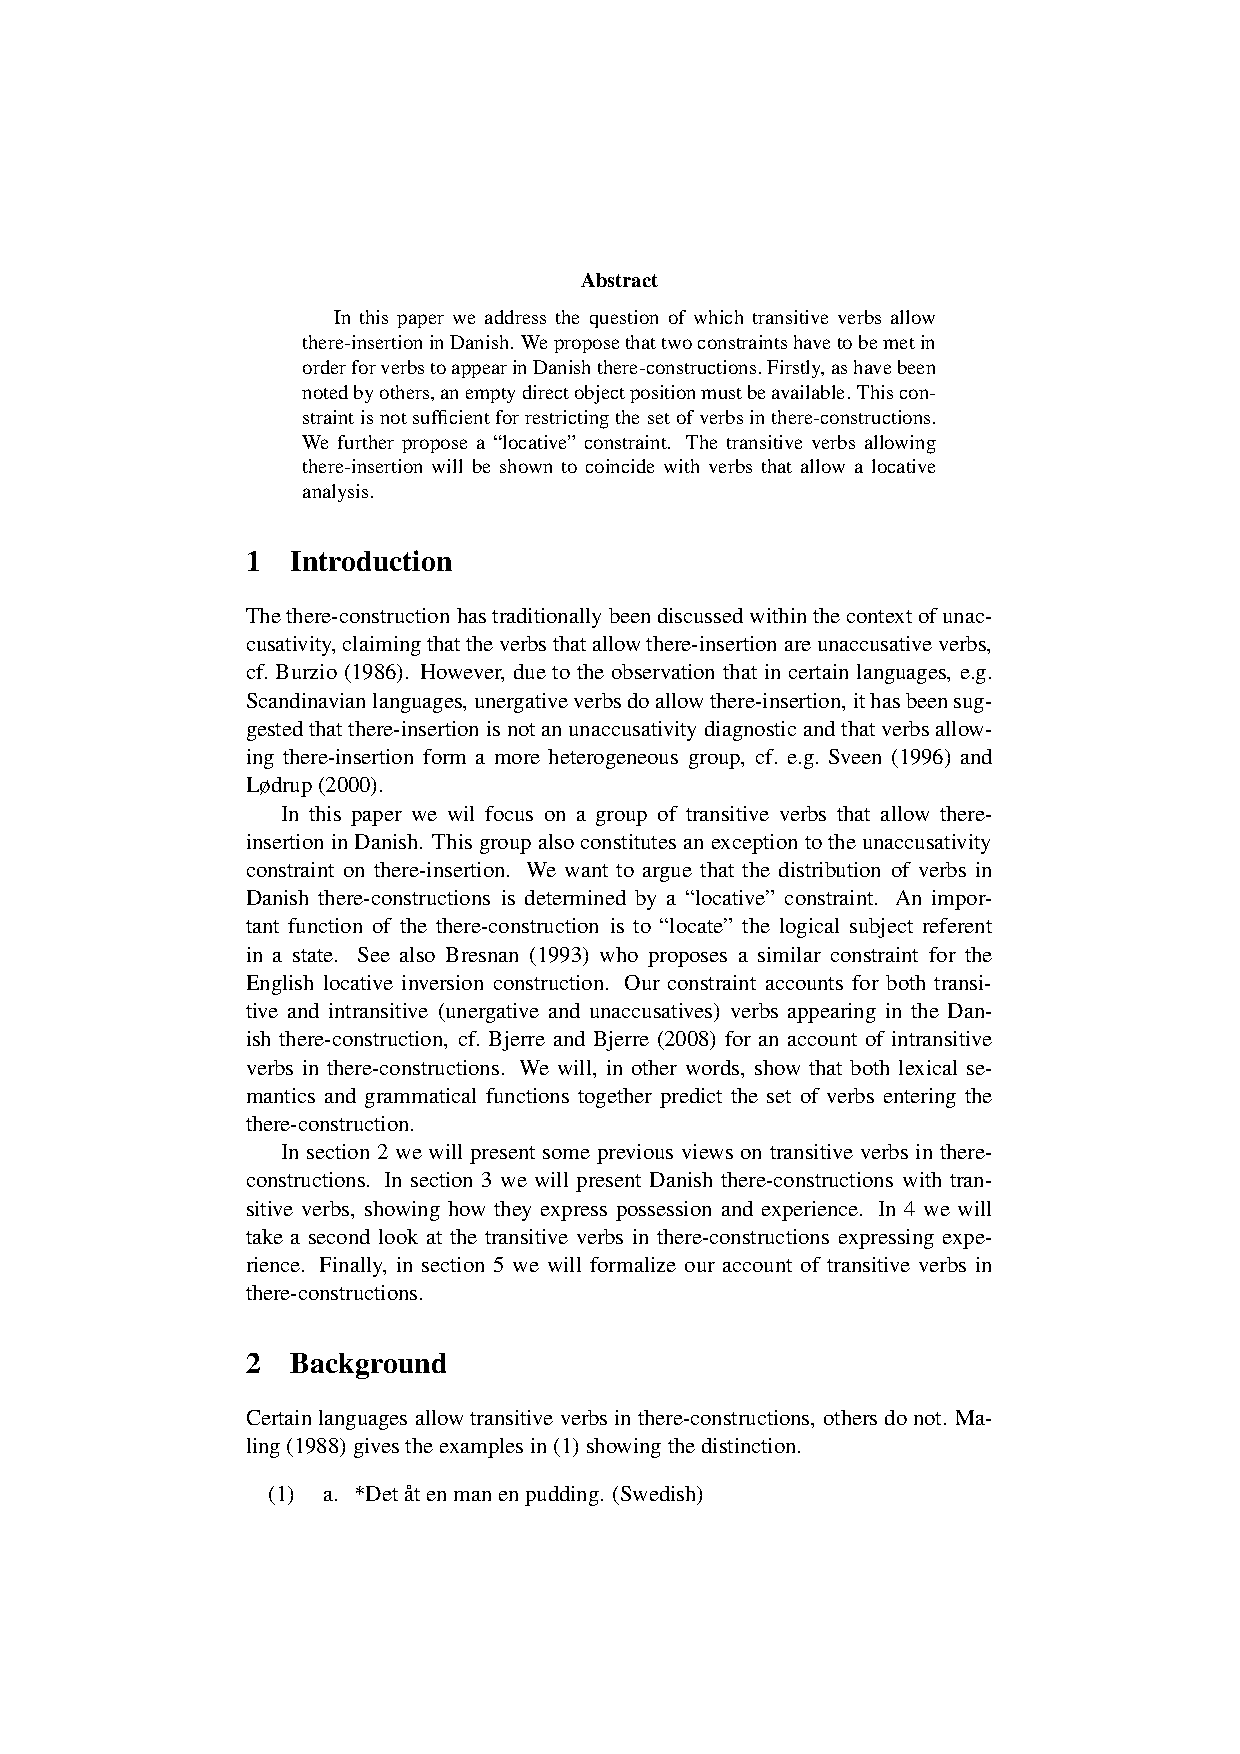
\includepdf[pages=-,pagecommand=\thispagestyle{plain}]{Includes/bjerre-bjerre.pdf}
        \setcounter{page}{67}
        \phantomsection
        \addcontentsline{toc}{section}{Scott Drellishak: Complex Case Phenomena in the Grammar Matrix}
\thispagestyle{empty}

\begin{center}
  {\huge\bfseries Complex Case Phenomena in the Grammar Matrix\par}

  \bigskip

~\\
\begingroup
\setlength{\leftskip}{0pt plus 1fill}
\setlength{\rightskip}{0pt plus 1fill}
\setlength{\parindent}{0pt}
\setlength{\parfillskip}{0pt}
  \formatauthor{Scott Drellishak}{\begin{tabular}{@{}c@{}}University of Washington\end{tabular}}

\par\endgroup

  \vspace*{8ex}

  Proceedings of the 15th International Conference on\par Head-Driven Phrase Structure Grammar

  \bigskip

  National Institute of Information and Communications Technology, Keihanna

  \medskip

  Stefan Müller (Editor)

  \medskip

  2008

  \medskip

  CSLI Publications

  \medskip

  pages 67--86

  \medskip

  \url{http://csli-publications.stanford.edu/HPSG/2008}
\end{center}
\vfill

\noindent



\vfill
\noindent
% APA Style
Drellishak, Scott. 2008. Complex Case Phenomena in the Grammar Matrix. In Müller, Stefan (Ed.), \emph{{Proceedings of the 15th International Conference on Head-Driven Phrase Structure Grammar, National Institute of Information and Communications Technology, Keihanna}}, 67--86. Stanford,
CA: CSLI Publications. \hfill\href{http://creativecommons.org/licenses/by/4.0/}{\includegraphics[height=.75em]{Includes/ccby.eps}}

\newpage
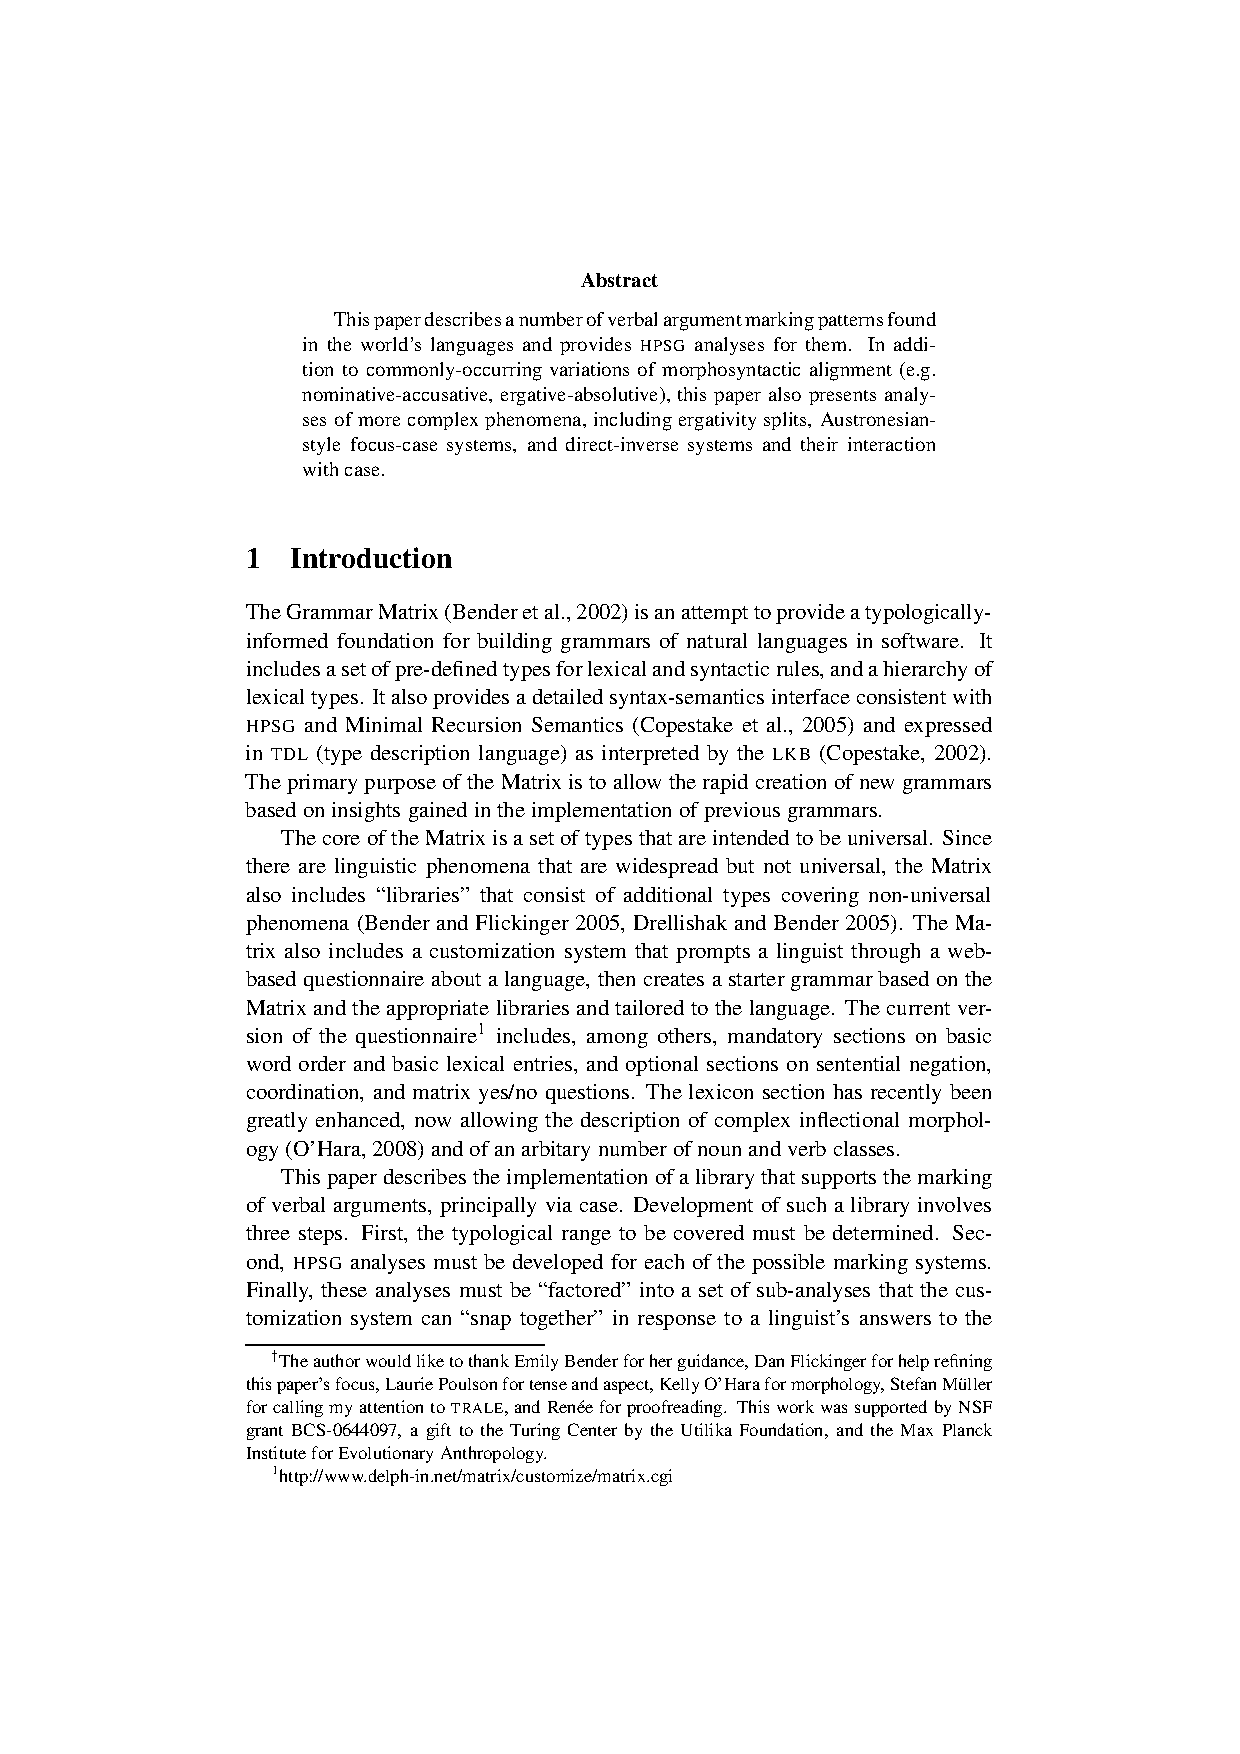
\includepdf[pages=-,pagecommand=\thispagestyle{plain}]{Includes/drellishak.pdf}
        \setcounter{page}{87}
        \phantomsection
        \addcontentsline{toc}{section}{Dan Flickinger: Transparent Heads}
\thispagestyle{empty}

\begin{center}
  {\huge\bfseries Transparent Heads\par}

  \bigskip

~\\
\begingroup
\setlength{\leftskip}{0pt plus 1fill}
\setlength{\rightskip}{0pt plus 1fill}
\setlength{\parindent}{0pt}
\setlength{\parfillskip}{0pt}
  \formatauthor{Dan Flickinger}{\begin{tabular}{@{}c@{}}CSLI, Stanford University\end{tabular}}

\par\endgroup

  \vspace*{8ex}

  Proceedings of the 15th International Conference on\par Head-Driven Phrase Structure Grammar

  \bigskip

  National Institute of Information and Communications Technology, Keihanna

  \medskip

  Stefan Müller (Editor)

  \medskip

  2008

  \medskip

  CSLI Publications

  \medskip

  pages 87--94

  \medskip

  \url{http://csli-publications.stanford.edu/HPSG/2008}
\end{center}
\vfill

\noindent



\vfill
\noindent
% APA Style
Flickinger, Dan. 2008. Transparent Heads. In Müller, Stefan (Ed.), \emph{{Proceedings of the 15th International Conference on Head-Driven Phrase Structure Grammar, National Institute of Information and Communications Technology, Keihanna}}, 87--94. Stanford,
CA: CSLI Publications. \hfill\href{http://creativecommons.org/licenses/by/4.0/}{\includegraphics[height=.75em]{Includes/ccby.eps}}

\newpage
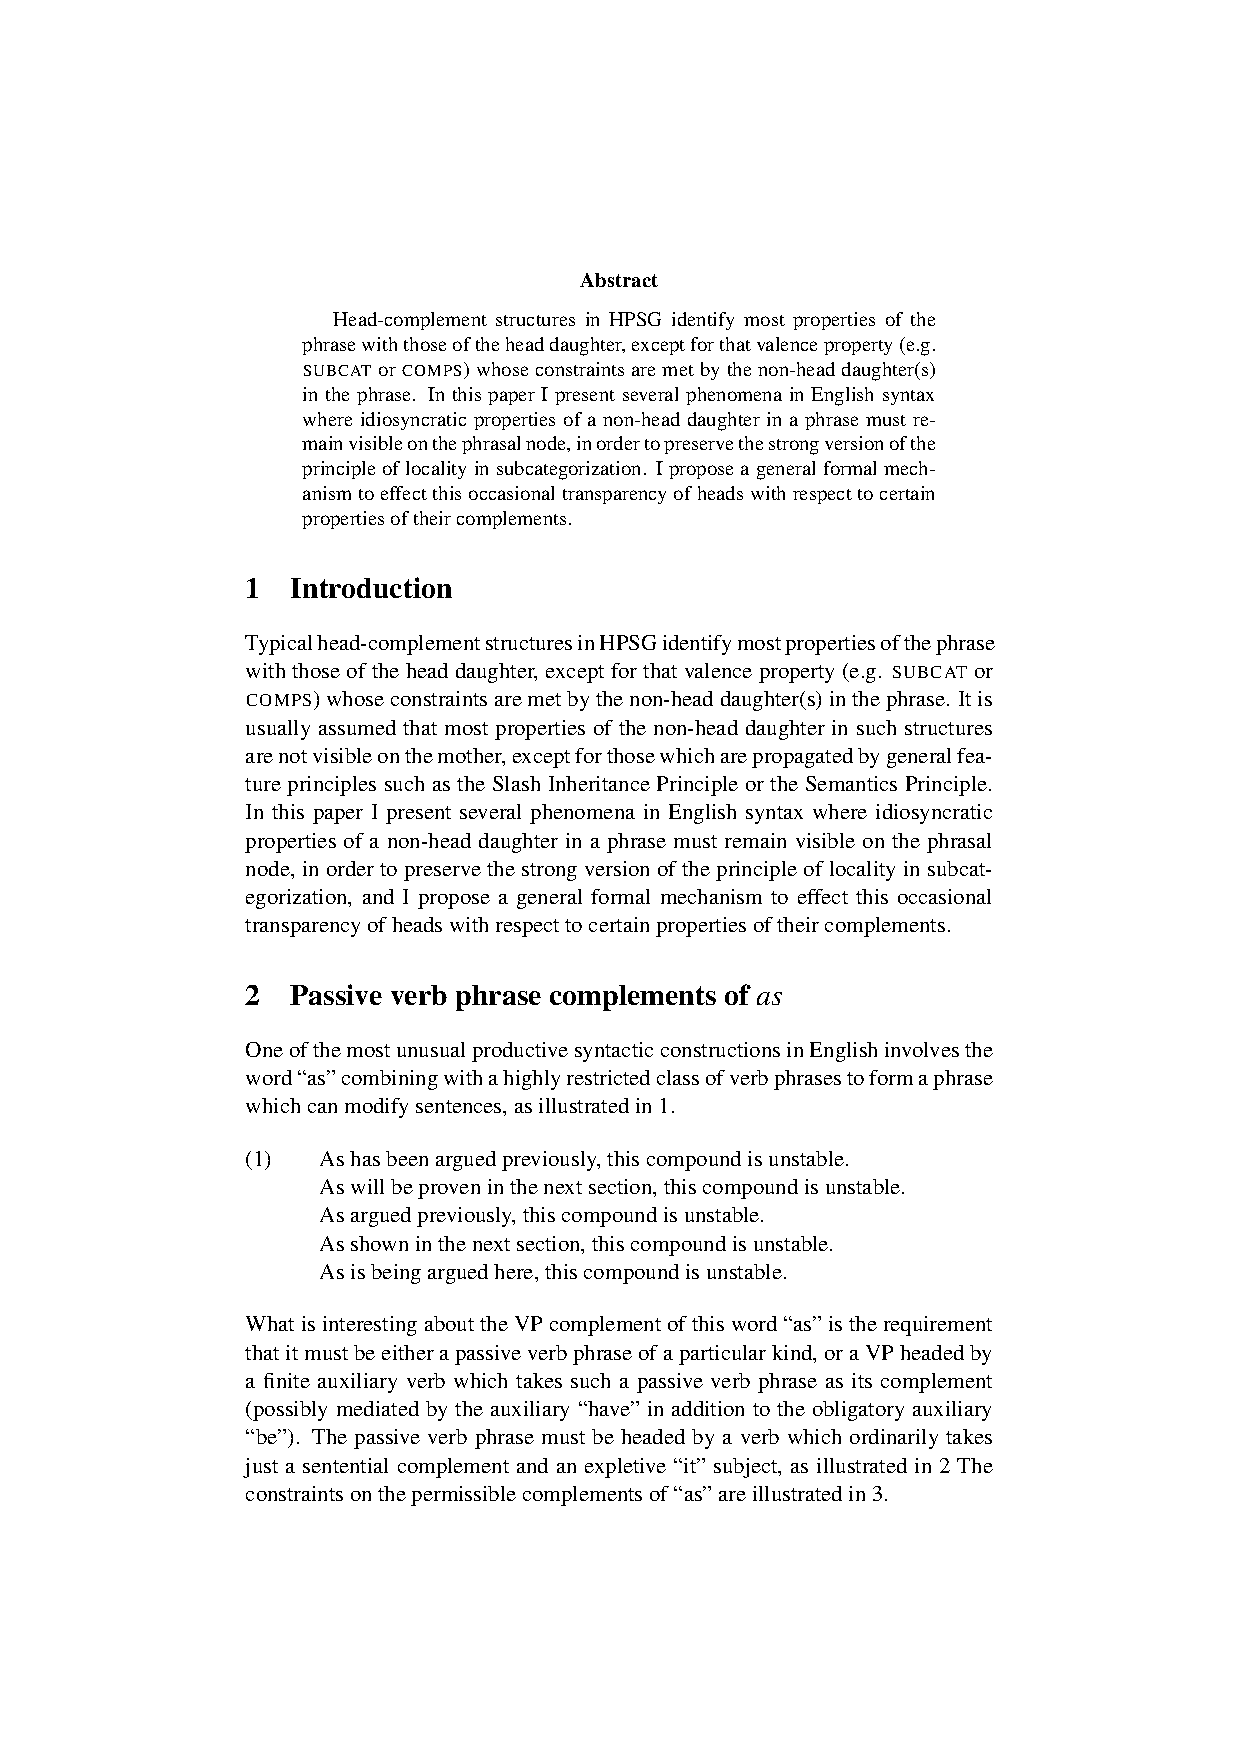
\includepdf[pages=-,pagecommand=\thispagestyle{plain}]{Includes/flickinger.pdf}
        \setcounter{page}{95}
        \phantomsection
        \addcontentsline{toc}{section}{Chizuru Ito, Rui P. Chaves: Apparent Non-Constituent Coordination in Japanese}
\thispagestyle{empty}

\begin{center}
  {\huge\bfseries Apparent Non-Constituent Coordination in Japanese\par}

  \bigskip

~\\
\begingroup
\setlength{\leftskip}{0pt plus 1fill}
\setlength{\rightskip}{0pt plus 1fill}
\setlength{\parindent}{0pt}
\setlength{\parfillskip}{0pt}
  \formatauthor{Chizuru Ito}{\begin{tabular}{@{}c@{}}Osaka University\end{tabular}}
\formatauthor{Rui P. Chaves}{\begin{tabular}{@{}c@{}}Lisbon University\end{tabular}}

\par\endgroup

  \vspace*{8ex}

  Proceedings of the 15th International Conference on\par Head-Driven Phrase Structure Grammar

  \bigskip

  National Institute of Information and Communications Technology, Keihanna

  \medskip

  Stefan Müller (Editor)

  \medskip

  2008

  \medskip

  CSLI Publications

  \medskip

  pages 95--115

  \medskip

  \url{http://csli-publications.stanford.edu/HPSG/2008}
\end{center}
\vfill

\noindent



\vfill
\noindent
% APA Style
Ito, Chizuru, \& Chaves, Rui P. 2008. Apparent Non-Constituent Coordination in Japanese. In Müller, Stefan (Ed.), \emph{{Proceedings of the 15th International Conference on Head-Driven Phrase Structure Grammar, National Institute of Information and Communications Technology, Keihanna}}, 95--115. Stanford,
CA: CSLI Publications. \hfill\href{http://creativecommons.org/licenses/by/4.0/}{\includegraphics[height=.75em]{Includes/ccby.eps}}

\newpage
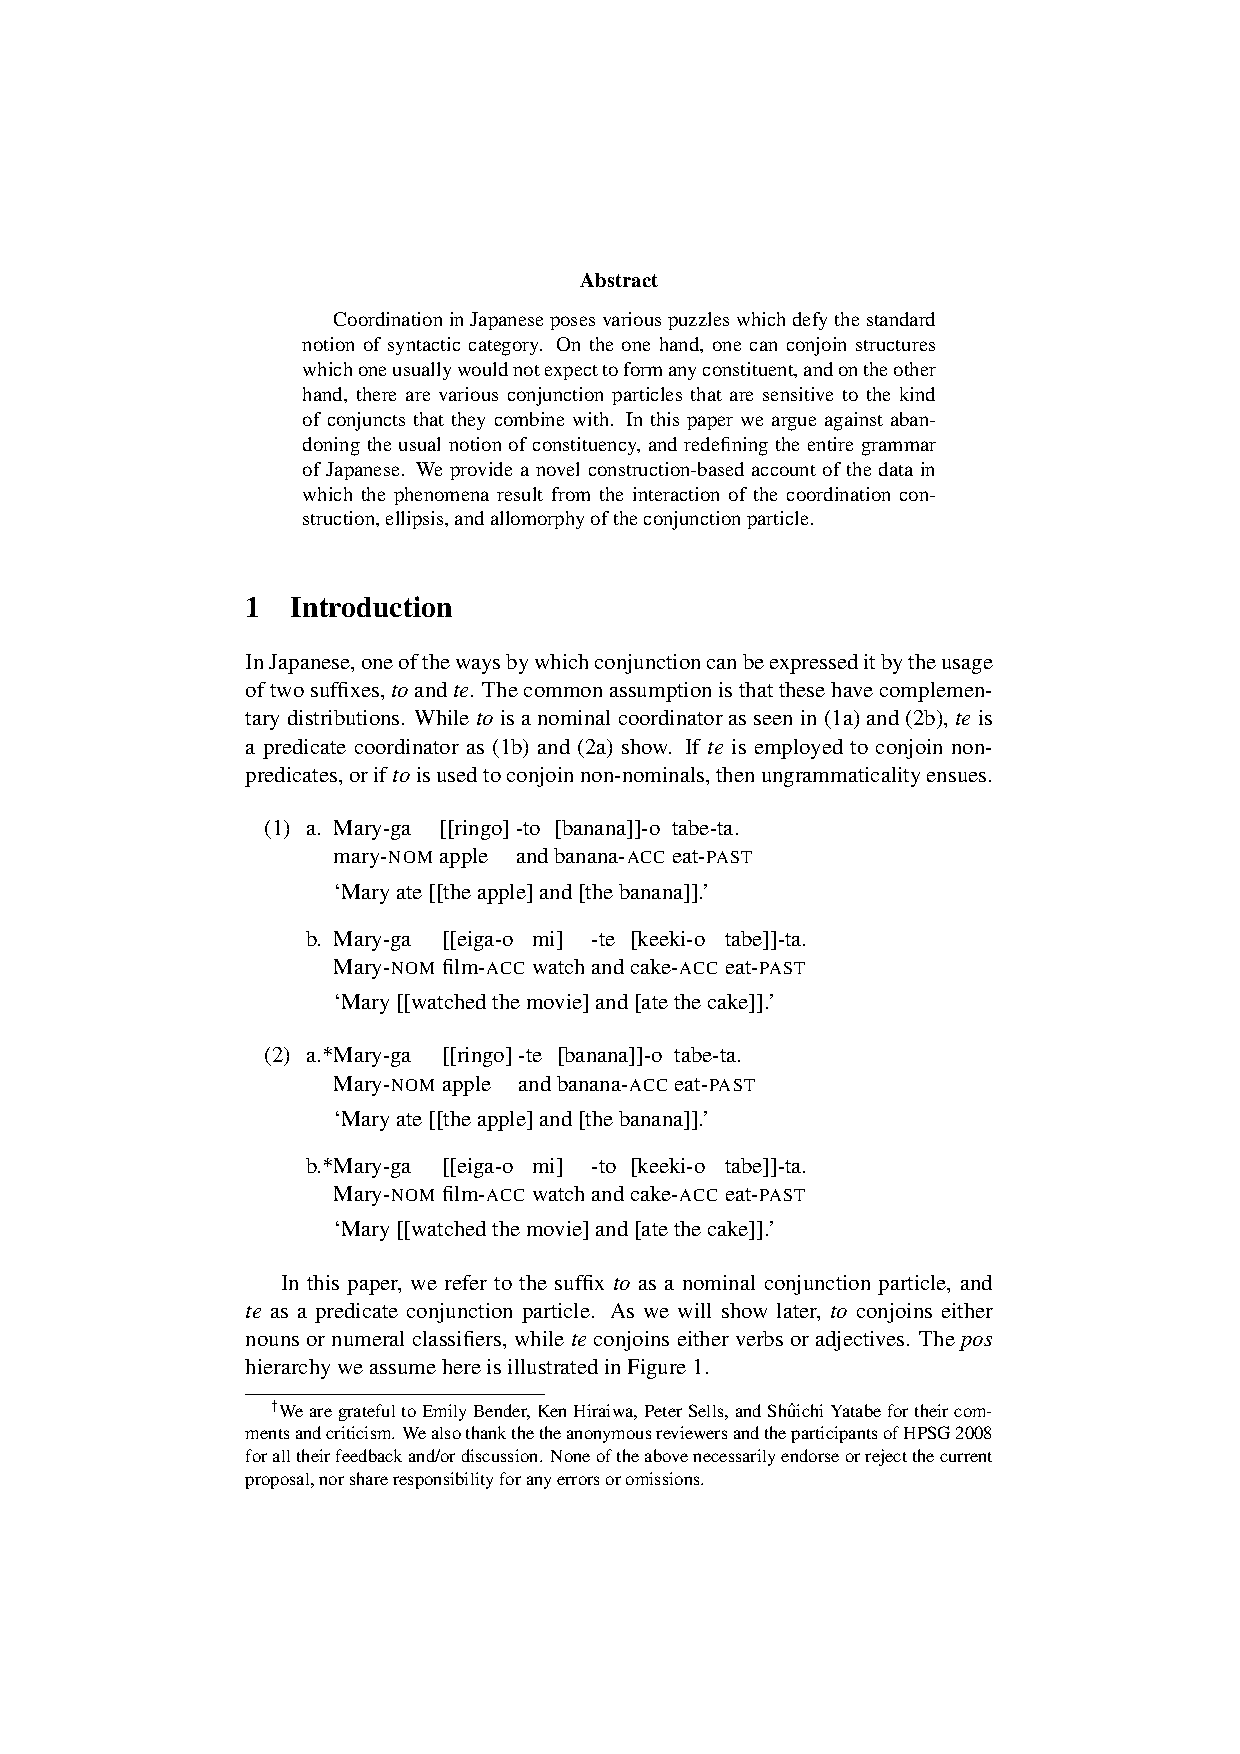
\includepdf[pages=-,pagecommand=\thispagestyle{plain}]{Includes/ito-chaves.pdf}
        \setcounter{page}{116}
        \phantomsection
        \addcontentsline{toc}{section}{Tibor Kiss: Towards a Grammar of Preposition-Noun Combinations}
\thispagestyle{empty}

\begin{center}
  {\huge\bfseries Towards a Grammar of Preposition-Noun Combinations\par}

  \bigskip

~\\
\begingroup
\setlength{\leftskip}{0pt plus 1fill}
\setlength{\rightskip}{0pt plus 1fill}
\setlength{\parindent}{0pt}
\setlength{\parfillskip}{0pt}
  \formatauthor{Tibor Kiss}{\begin{tabular}{@{}c@{}}Ruhr-Universität Bochum\end{tabular}}

\par\endgroup

  \vspace*{8ex}

  Proceedings of the 15th International Conference on\par Head-Driven Phrase Structure Grammar

  \bigskip

  National Institute of Information and Communications Technology, Keihanna

  \medskip

  Stefan Müller (Editor)

  \medskip

  2008

  \medskip

  CSLI Publications

  \medskip

  pages 116--130

  \medskip

  \url{http://csli-publications.stanford.edu/HPSG/2008}
\end{center}
\vfill

\noindent



\vfill
\noindent
% APA Style
Kiss, Tibor. 2008. Towards a Grammar of Preposition-Noun Combinations. In Müller, Stefan (Ed.), \emph{{Proceedings of the 15th International Conference on Head-Driven Phrase Structure Grammar, National Institute of Information and Communications Technology, Keihanna}}, 116--130. Stanford,
CA: CSLI Publications. \hfill\href{http://creativecommons.org/licenses/by/4.0/}{\includegraphics[height=.75em]{Includes/ccby.eps}}

\newpage
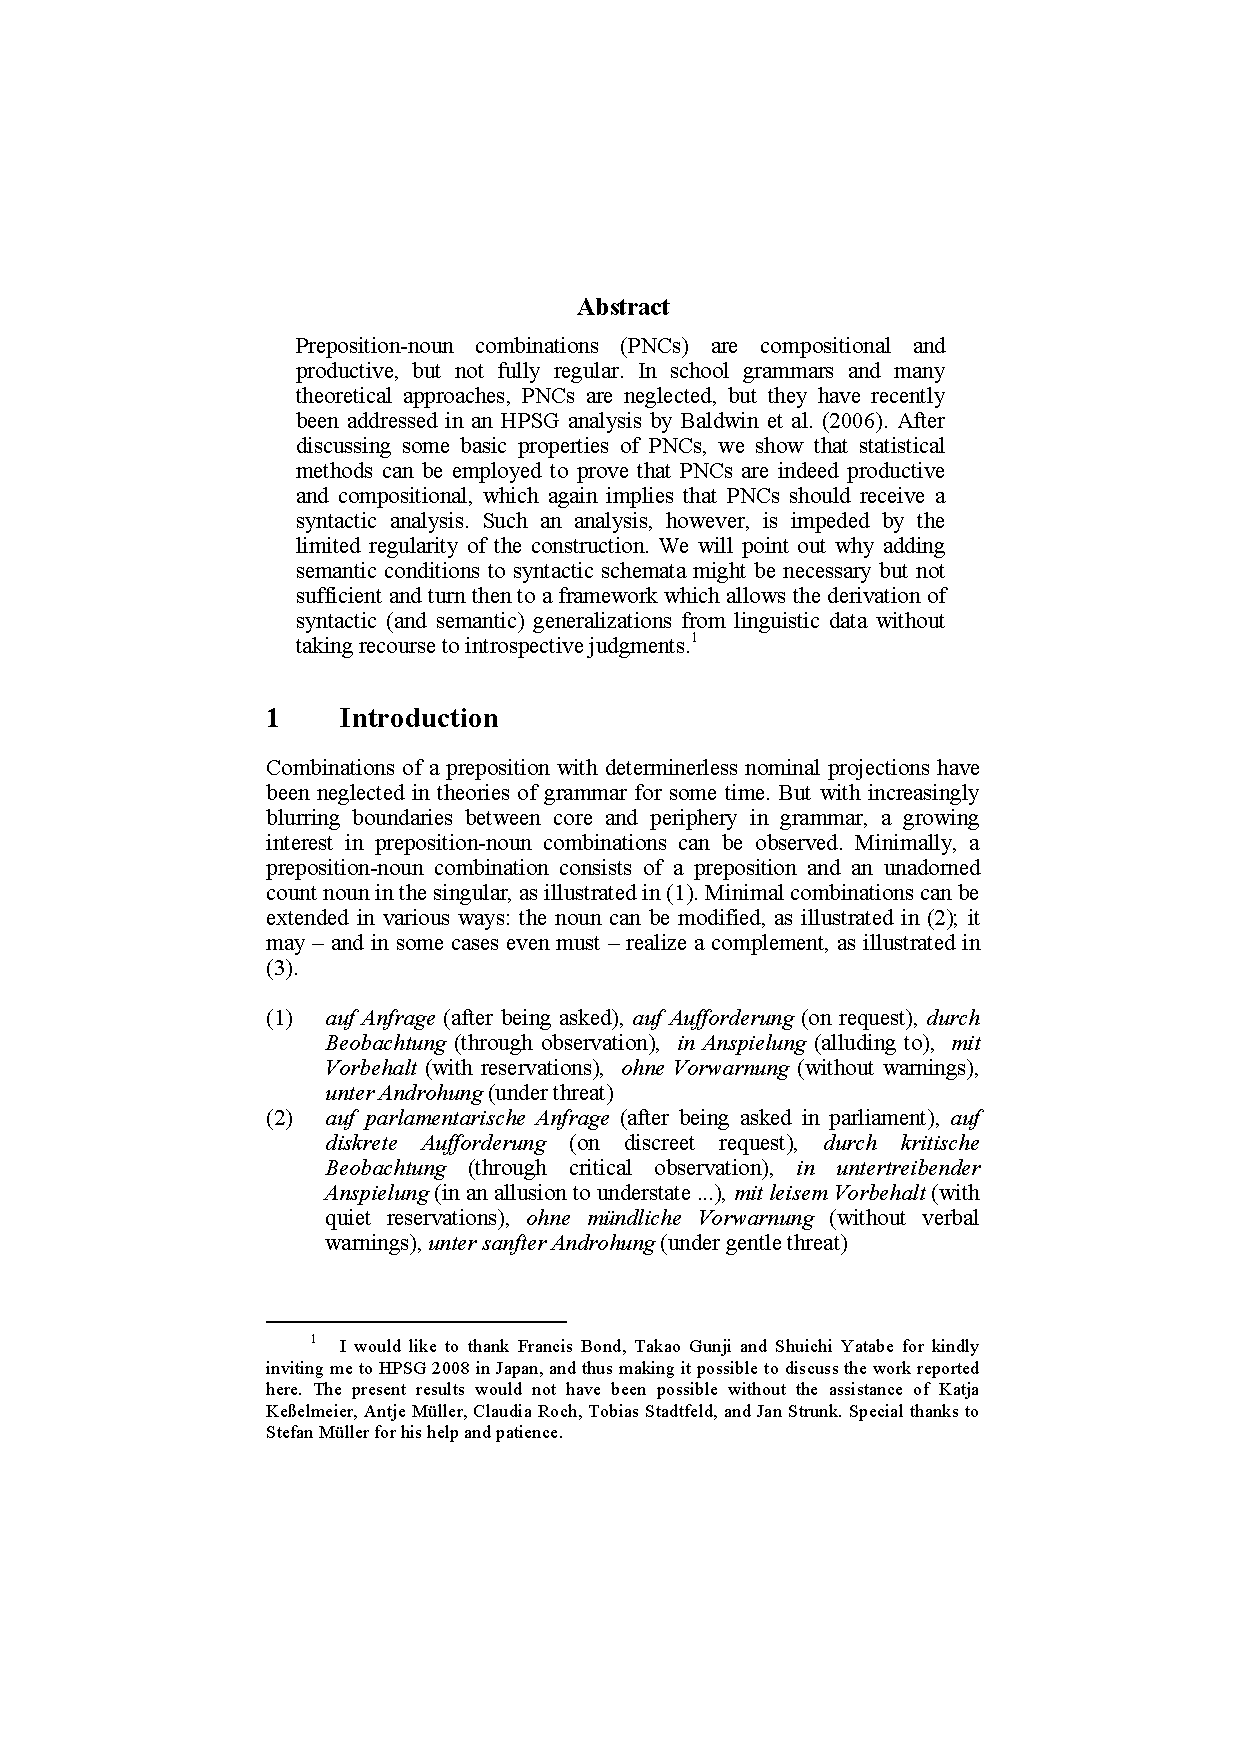
\includepdf[pages=-,pagecommand=\thispagestyle{plain}]{Includes/kiss.pdf}
        \setcounter{page}{131}
        \phantomsection
        \addcontentsline{toc}{section}{Kil Soo Ko: Korean Postpositions as Weak Syntactic Heads}
\thispagestyle{empty}

\begin{center}
  {\huge\bfseries Korean Postpositions as Weak Syntactic Heads\par}

  \bigskip

~\\
\begingroup
\setlength{\leftskip}{0pt plus 1fill}
\setlength{\rightskip}{0pt plus 1fill}
\setlength{\parindent}{0pt}
\setlength{\parfillskip}{0pt}
  \formatauthor{Kil Soo Ko}{\begin{tabular}{@{}c@{}}University Paris 7\end{tabular}}

\par\endgroup

  \vspace*{8ex}

  Proceedings of the 15th International Conference on\par Head-Driven Phrase Structure Grammar

  \bigskip

  National Institute of Information and Communications Technology, Keihanna

  \medskip

  Stefan Müller (Editor)

  \medskip

  2008

  \medskip

  CSLI Publications

  \medskip

  pages 131--151

  \medskip

  \url{http://csli-publications.stanford.edu/HPSG/2008}
\end{center}
\vfill

\noindent



\vfill
\noindent
% APA Style
Ko, Kil Soo. 2008. Korean Postpositions as Weak Syntactic Heads. In Müller, Stefan (Ed.), \emph{{Proceedings of the 15th International Conference on Head-Driven Phrase Structure Grammar, National Institute of Information and Communications Technology, Keihanna}}, 131--151. Stanford,
CA: CSLI Publications. \hfill\href{http://creativecommons.org/licenses/by/4.0/}{\includegraphics[height=.75em]{Includes/ccby.eps}}

\newpage
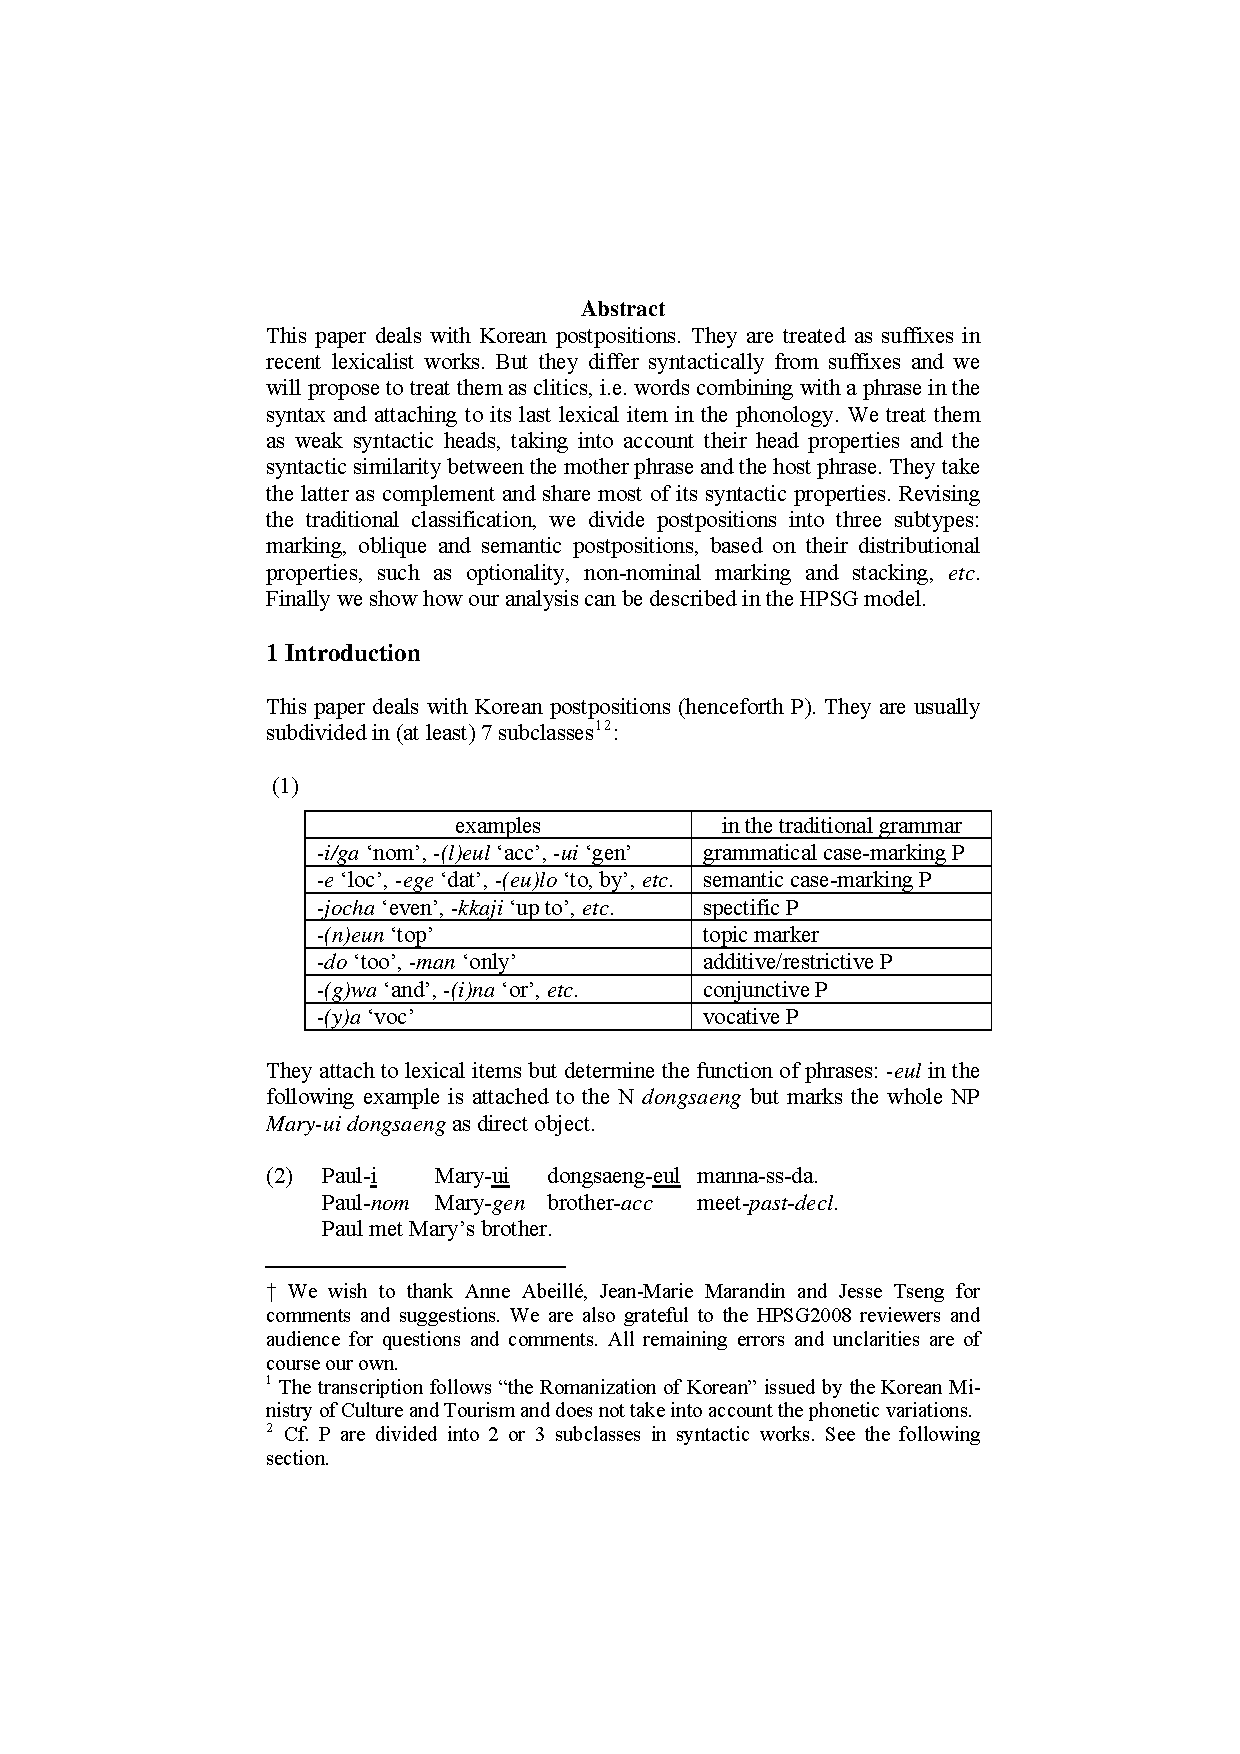
\includepdf[pages=-,pagecommand=\thispagestyle{plain}]{Includes/ko.pdf}
        \setcounter{page}{152}
        \phantomsection
        \addcontentsline{toc}{section}{Fr{\'e}d{\'e}ric Laurens: French Predicative Verbless Utterances}
\thispagestyle{empty}

\begin{center}
  {\huge\bfseries French Predicative Verbless Utterances\par}

  \bigskip

~\\
\begingroup
\setlength{\leftskip}{0pt plus 1fill}
\setlength{\rightskip}{0pt plus 1fill}
\setlength{\parindent}{0pt}
\setlength{\parfillskip}{0pt}
  \formatauthor{Frédéric Laurens}{\begin{tabular}{@{}c@{}}Université Paris 7\end{tabular}}

\par\endgroup

  \vspace*{8ex}

  Proceedings of the 15th International Conference on\par Head-Driven Phrase Structure Grammar

  \bigskip

  National Institute of Information and Communications Technology, Keihanna

  \medskip

  Stefan Müller (Editor)

  \medskip

  2008

  \medskip

  CSLI Publications

  \medskip

  pages 152--172

  \medskip

  \url{http://csli-publications.stanford.edu/HPSG/2008}
\end{center}
\vfill

\noindent



\vfill
\noindent
% APA Style
Laurens, Frédéric. 2008. French Predicative Verbless Utterances. In Müller, Stefan (Ed.), \emph{{Proceedings of the 15th International Conference on Head-Driven Phrase Structure Grammar, National Institute of Information and Communications Technology, Keihanna}}, 152--172. Stanford,
CA: CSLI Publications. \hfill\href{http://creativecommons.org/licenses/by/4.0/}{\includegraphics[height=.75em]{Includes/ccby.eps}}

\newpage
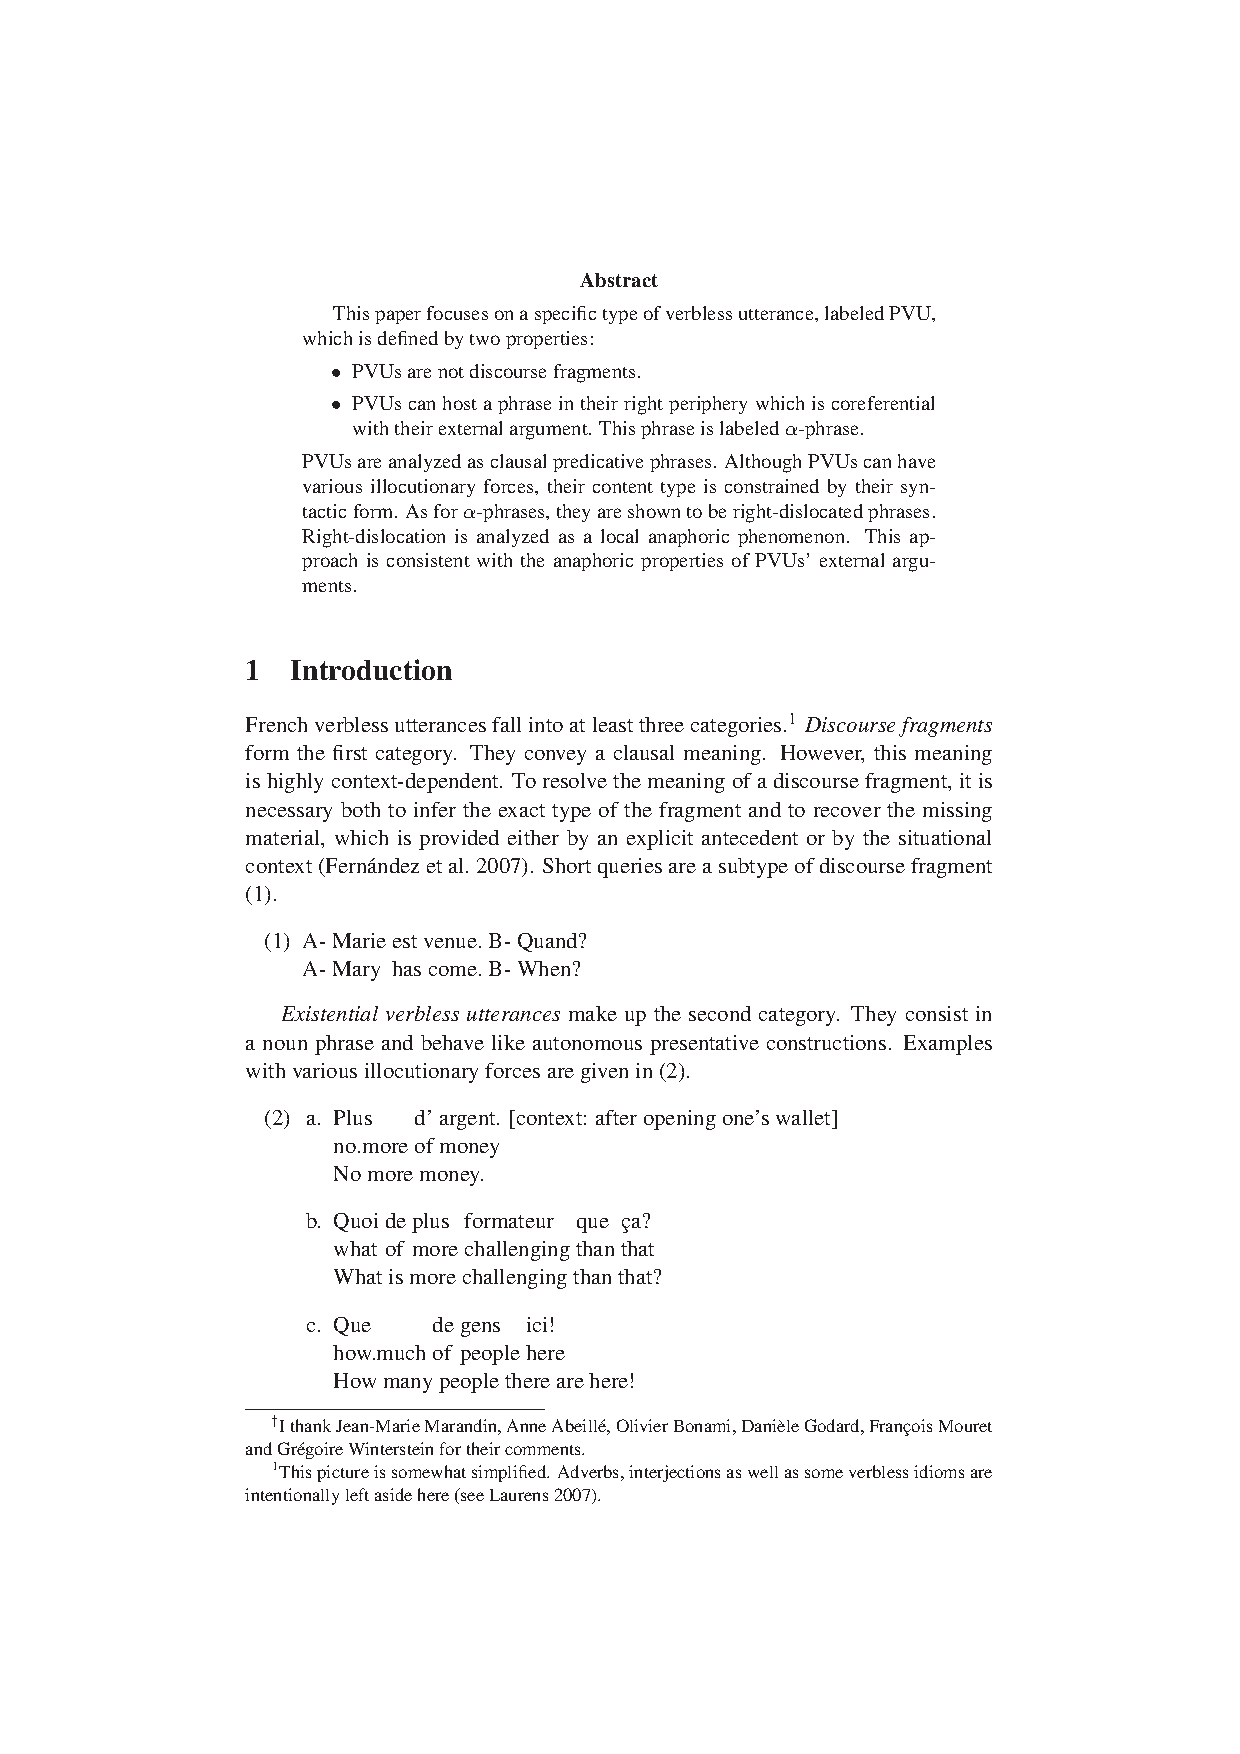
\includepdf[pages=-,pagecommand=\thispagestyle{plain}]{Includes/laurens.pdf}
        \setcounter{page}{173}
        \phantomsection
        \addcontentsline{toc}{section}{Yo Sato, Wai Lok Tam: Towards a Unified Account of Adjuncts}
\thispagestyle{empty}

\begin{center}
  {\huge\bfseries Towards a Unified Account of Adjuncts\par}

  \bigskip

~\\
\begingroup
\setlength{\leftskip}{0pt plus 1fill}
\setlength{\rightskip}{0pt plus 1fill}
\setlength{\parindent}{0pt}
\setlength{\parfillskip}{0pt}
  \formatauthor{Yo Sato}{\begin{tabular}{@{}c@{}}King's College \\ Queen Mary University of London\end{tabular}}
\formatauthor{Wai Lok Tam}{\begin{tabular}{@{}c@{}}Tokyo University\end{tabular}}

\par\endgroup

  \vspace*{8ex}

  Proceedings of the 15th International Conference on\par Head-Driven Phrase Structure Grammar

  \bigskip

  National Institute of Information and Communications Technology, Keihanna

  \medskip

  Stefan Müller (Editor)

  \medskip

  2008

  \medskip

  CSLI Publications

  \medskip

  pages 173--188

  \medskip

  \url{http://csli-publications.stanford.edu/HPSG/2008}
\end{center}
\vfill

\noindent



\vfill
\noindent
% APA Style
Sato, Yo, \& Tam, Wai Lok. 2008. Towards a Unified Account of Adjuncts. In Müller, Stefan (Ed.), \emph{{Proceedings of the 15th International Conference on Head-Driven Phrase Structure Grammar, National Institute of Information and Communications Technology, Keihanna}}, 173--188. Stanford,
CA: CSLI Publications. \hfill\href{http://creativecommons.org/licenses/by/4.0/}{\includegraphics[height=.75em]{Includes/ccby.eps}}

\newpage
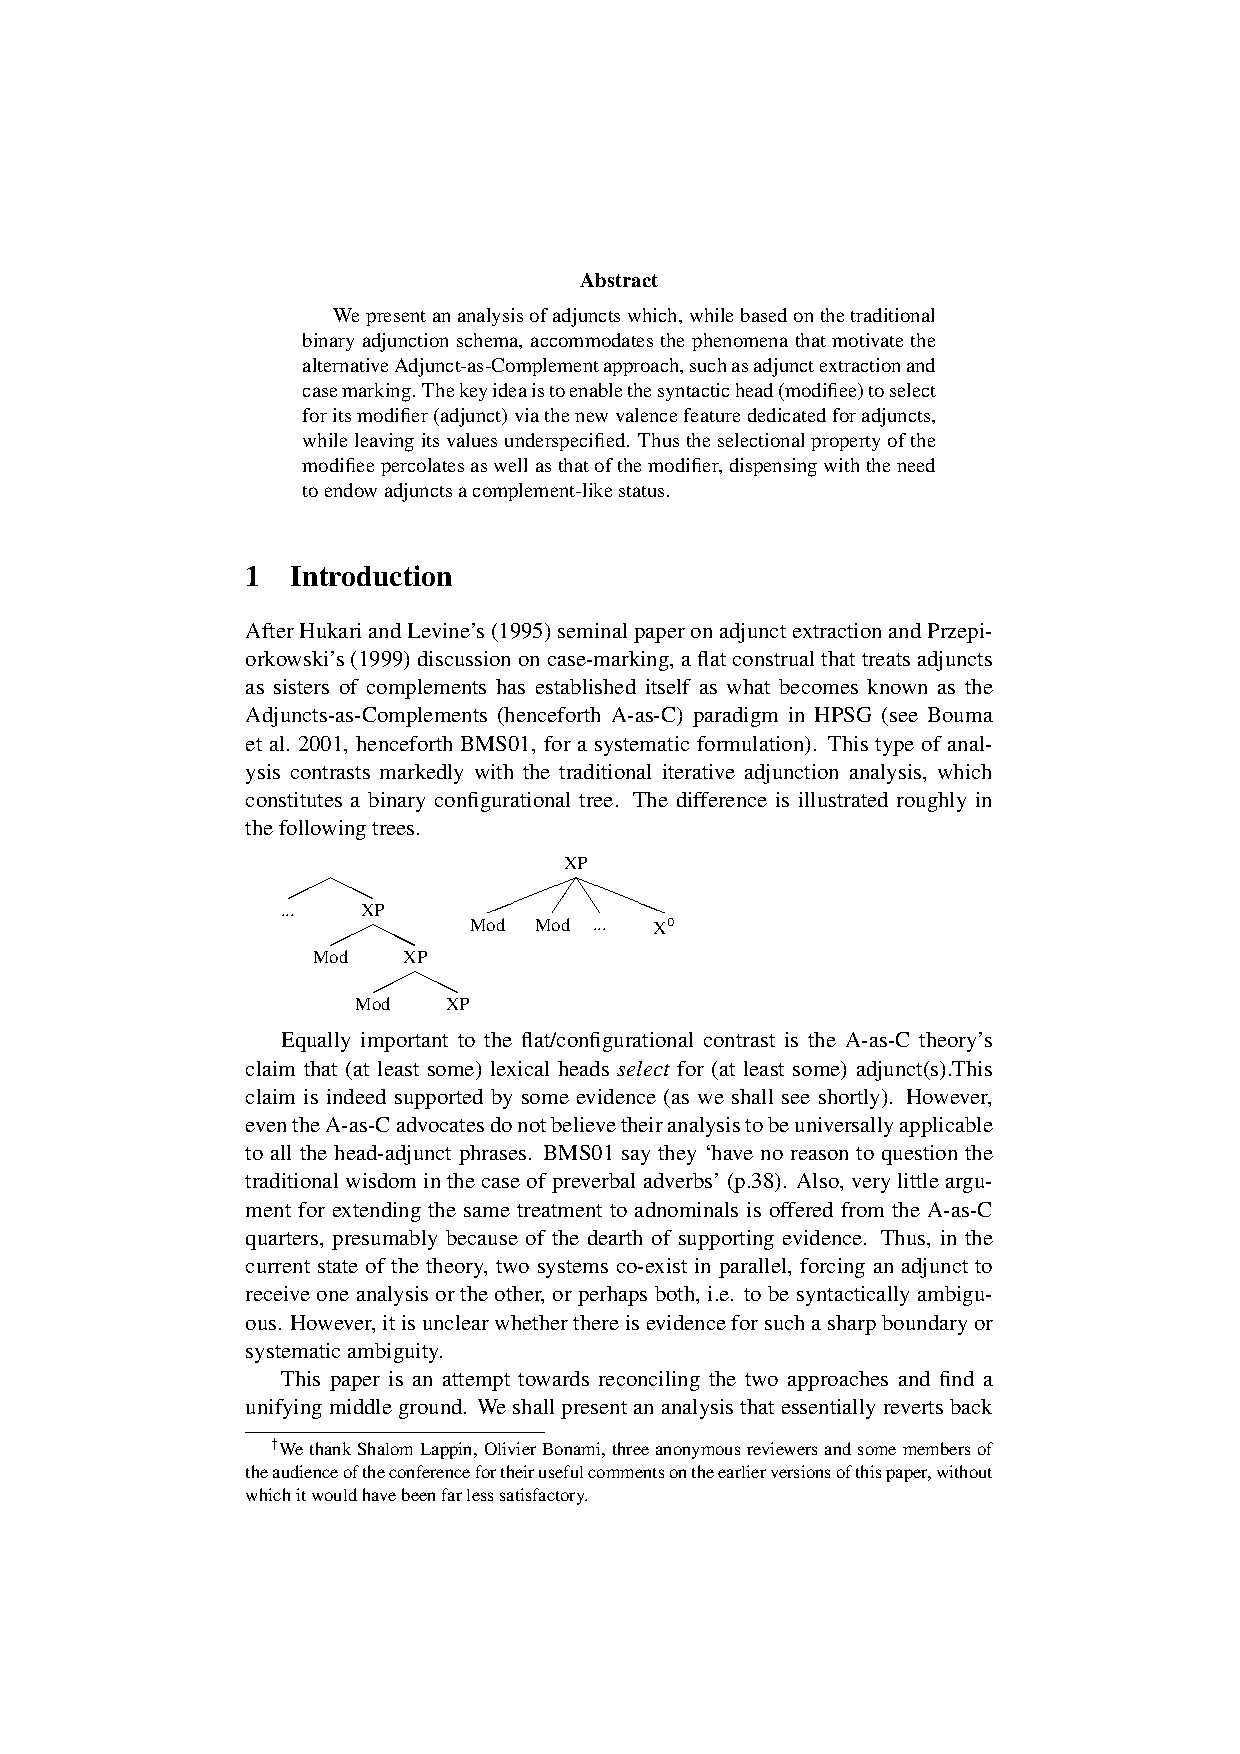
\includepdf[pages=-,pagecommand=\thispagestyle{plain}]{Includes/sato-tam.pdf}
        \setcounter{page}{189}
        \phantomsection
        \addcontentsline{toc}{section}{Karen Steinicke, Gerald Penn: Memory Management for Unification-based Processing of Typed Feature Structures}
\thispagestyle{empty}

\begin{center}
  {\huge\bfseries Memory Management for Unification-based Processing of Typed Feature Structures\par}

  \bigskip

~\\
\begingroup
\setlength{\leftskip}{0pt plus 1fill}
\setlength{\rightskip}{0pt plus 1fill}
\setlength{\parindent}{0pt}
\setlength{\parfillskip}{0pt}
  \formatauthor{Karen Steinicke}{\begin{tabular}{@{}c@{}}Universität Tübingen\end{tabular}}
\formatauthor{Gerald Penn}{\begin{tabular}{@{}c@{}}University of Toronto\end{tabular}}

\par\endgroup

  \vspace*{8ex}

  Proceedings of the 15th International Conference on\par Head-Driven Phrase Structure Grammar

  \bigskip

  National Institute of Information and Communications Technology, Keihanna

  \medskip

  Stefan Müller (Editor)

  \medskip

  2008

  \medskip

  CSLI Publications

  \medskip

  pages 189--203

  \medskip

  \url{http://csli-publications.stanford.edu/HPSG/2008}
\end{center}
\vfill

\noindent



\vfill
\noindent
% APA Style
Steinicke, Karen, \& Penn, Gerald. 2008. Memory Management for Unification-based Processing of Typed Feature Structures. In Müller, Stefan (Ed.), \emph{{Proceedings of the 15th International Conference on Head-Driven Phrase Structure Grammar, National Institute of Information and Communications Technology, Keihanna}}, 189--203. Stanford,
CA: CSLI Publications. \hfill\href{http://creativecommons.org/licenses/by/4.0/}{\includegraphics[height=.75em]{Includes/ccby.eps}}

\newpage
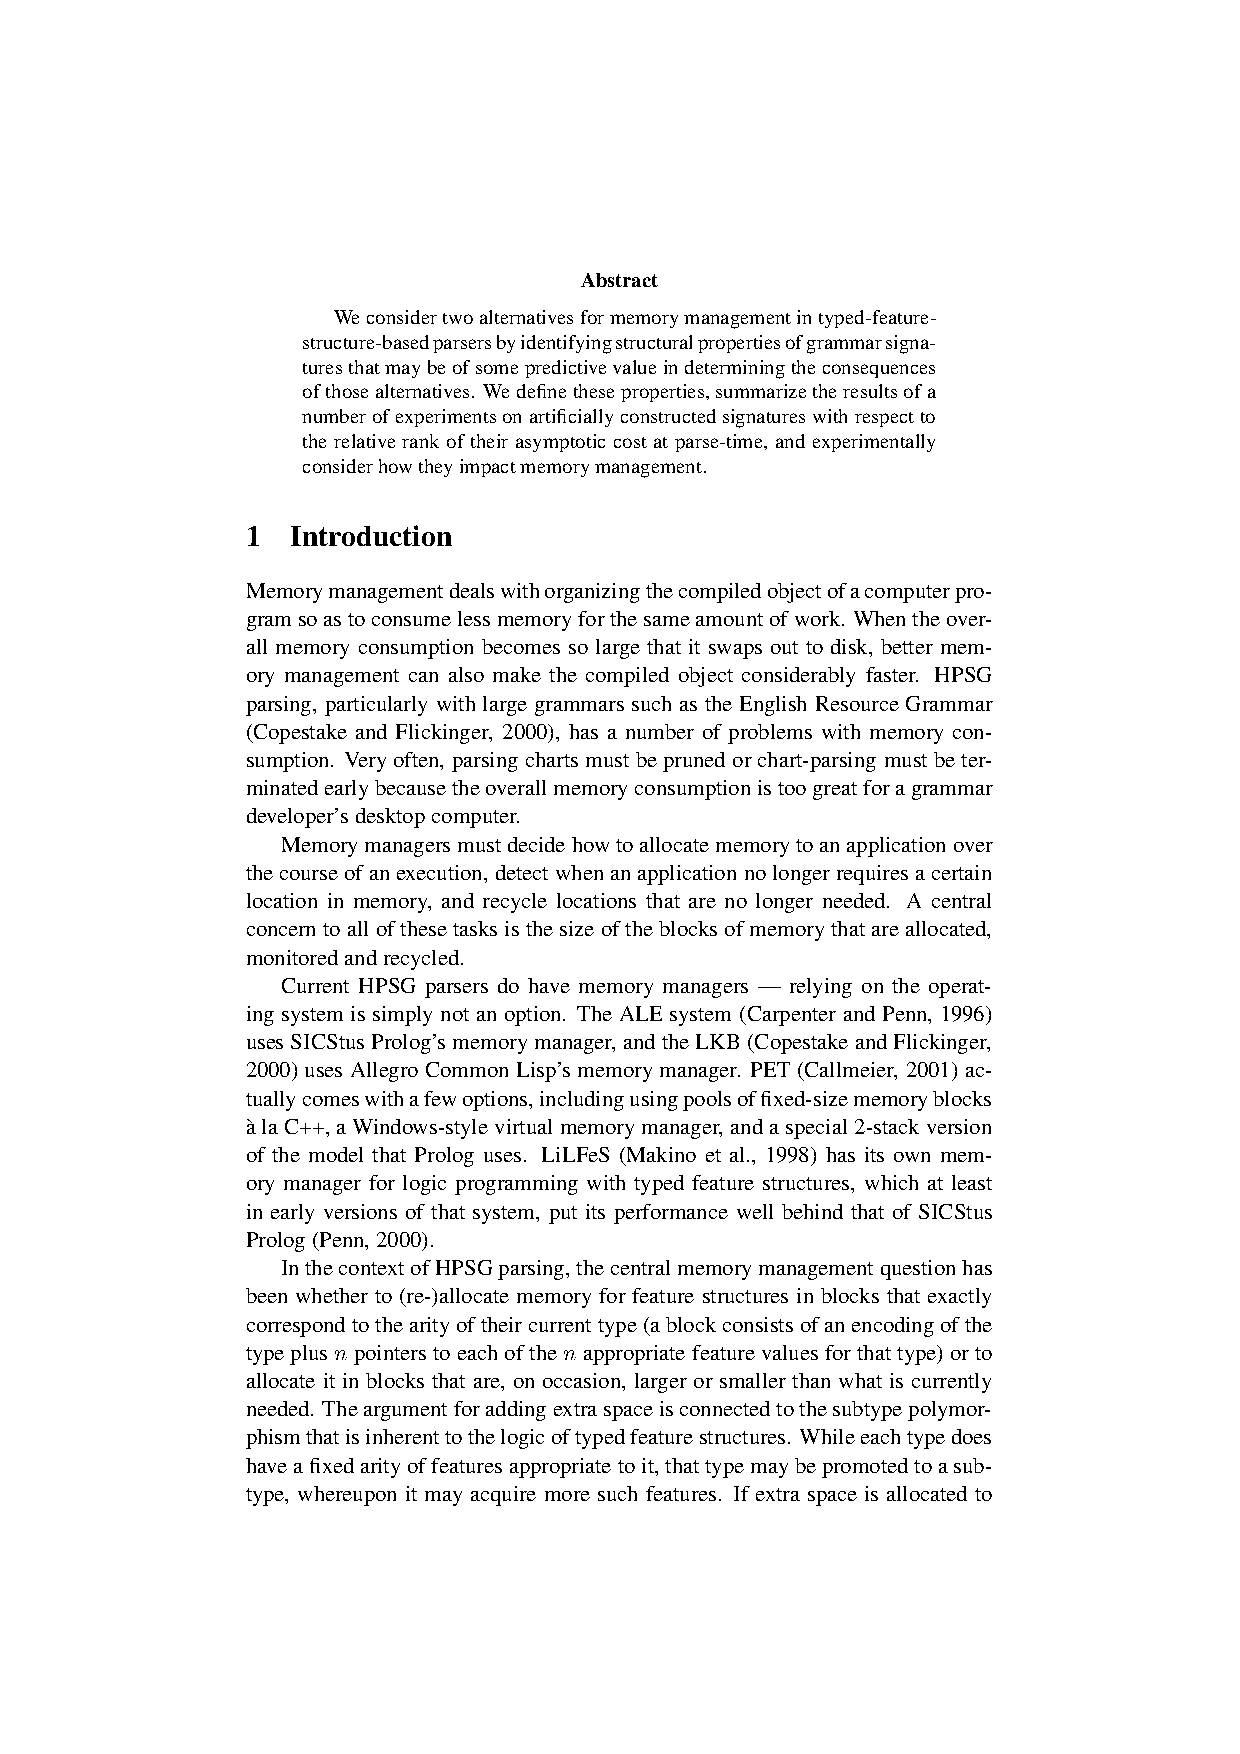
\includepdf[pages=-,pagecommand=\thispagestyle{plain}]{Includes/steinicke-penn.pdf}
        \setcounter{page}{204}
        \phantomsection
        \addcontentsline{toc}{section}{Sanghoun Song, Jae-Woong Choe: Automatic Construction of Korean Verbal Type Hierarchy using Treebank}
\thispagestyle{empty}

\begin{center}
  {\huge\bfseries Automatic Construction of Korean Verbal Type Hierarchy using Treebank\par}

  \bigskip

~\\
\begingroup
\setlength{\leftskip}{0pt plus 1fill}
\setlength{\rightskip}{0pt plus 1fill}
\setlength{\parindent}{0pt}
\setlength{\parfillskip}{0pt}
  \formatauthor{Sanghoun Song}{\begin{tabular}{@{}c@{}}Korea University\end{tabular}}
\formatauthor{Jae-Woong Choe}{\begin{tabular}{@{}c@{}}Korea University\end{tabular}}

\par\endgroup

  \vspace*{8ex}

  Proceedings of the 15th International Conference on\par Head-Driven Phrase Structure Grammar

  \bigskip

  National Institute of Information and Communications Technology, Keihanna

  \medskip

  Stefan Müller (Editor)

  \medskip

  2008

  \medskip

  CSLI Publications

  \medskip

  pages 204--221

  \medskip

  \url{http://csli-publications.stanford.edu/HPSG/2008}
\end{center}
\vfill

\noindent



\vfill
\noindent
% APA Style
Song, Sanghoun, \& Choe, Jae-Woong. 2008. Automatic Construction of Korean Verbal Type Hierarchy using Treebank. In Müller, Stefan (Ed.), \emph{{Proceedings of the 15th International Conference on Head-Driven Phrase Structure Grammar, National Institute of Information and Communications Technology, Keihanna}}, 204--221. Stanford,
CA: CSLI Publications. \hfill\href{http://creativecommons.org/licenses/by/4.0/}{\includegraphics[height=.75em]{Includes/ccby.eps}}

\newpage
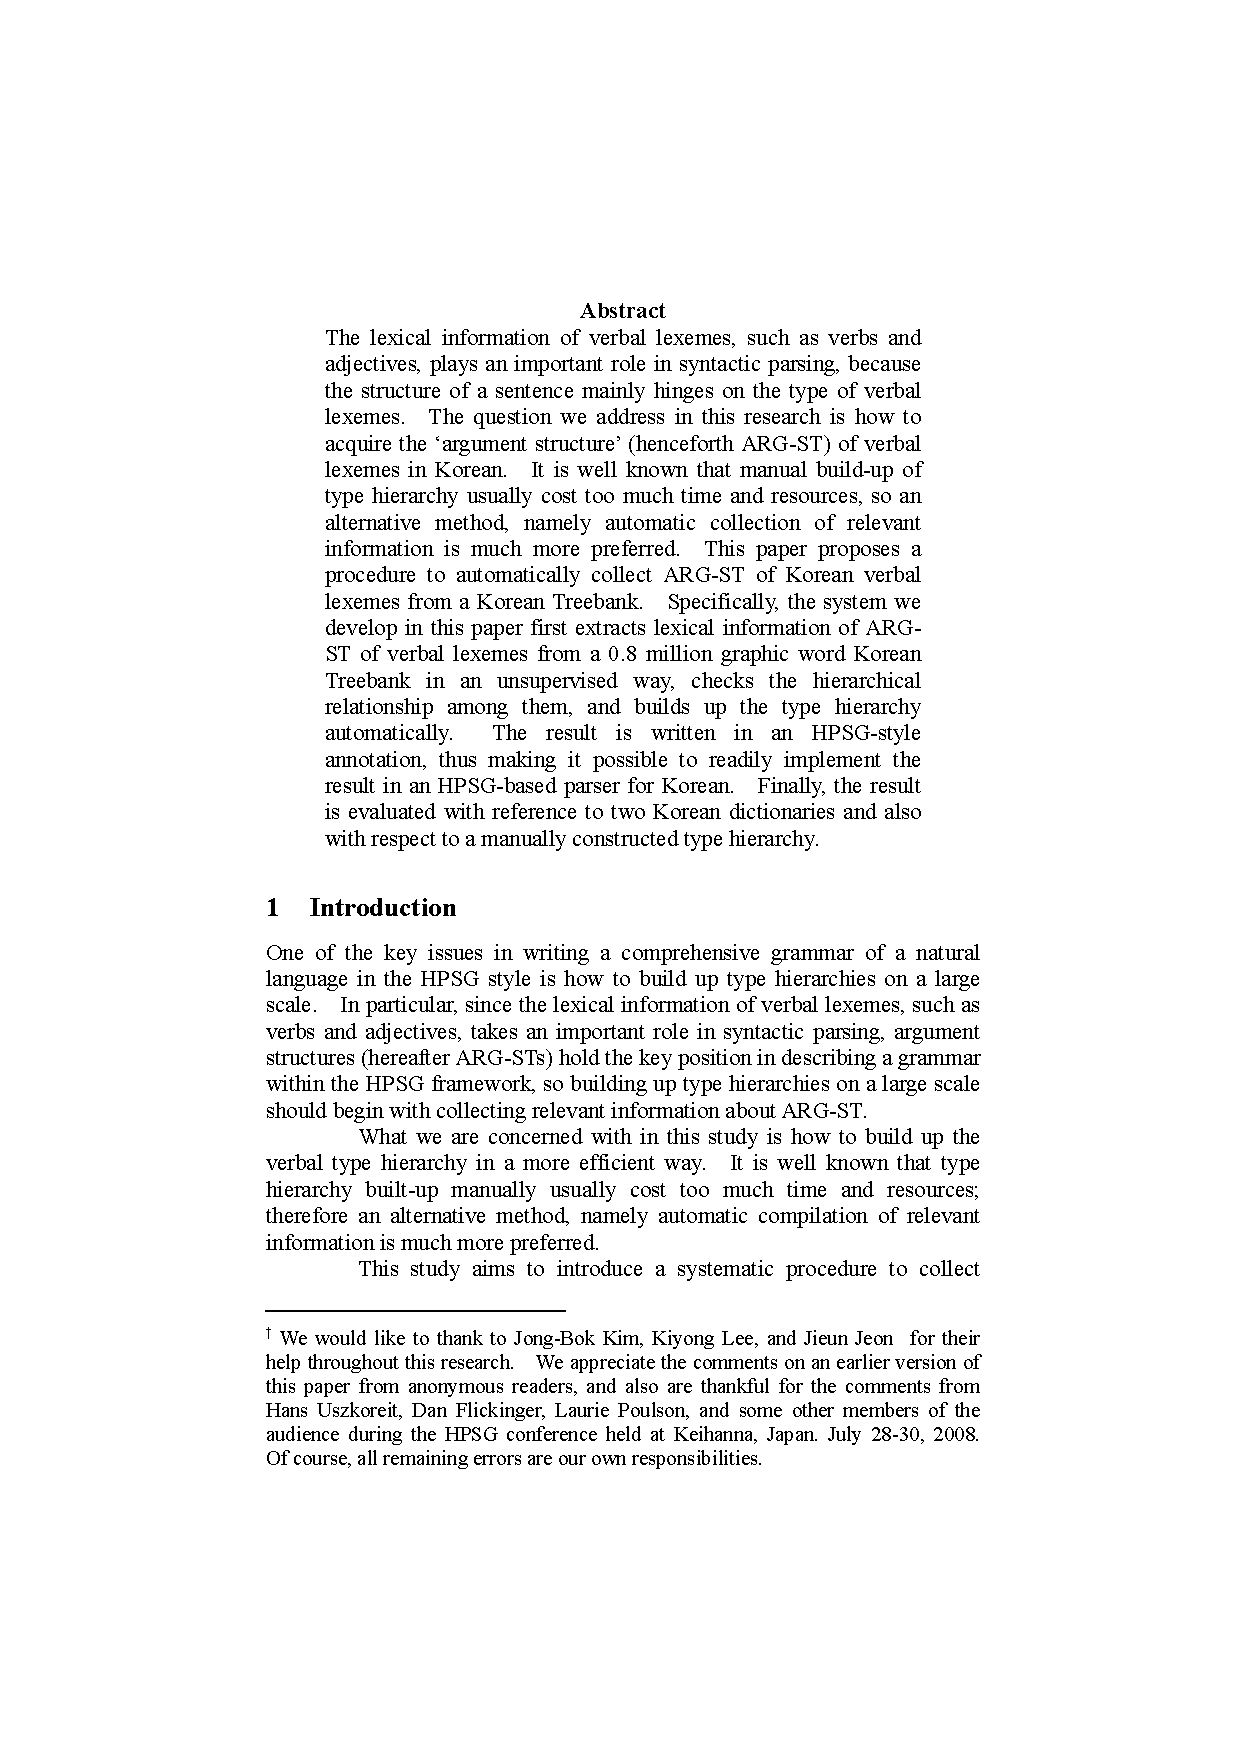
\includepdf[pages=-,pagecommand=\thispagestyle{plain}]{Includes/song-choe.pdf}
        \setcounter{page}{222}
        \phantomsection
        \addcontentsline{toc}{section}{Wai Lok Tam, Yo Sato: An Analysis of Pseudopartitives and Measure Phrases that Say
No to Extra Rules}
\thispagestyle{empty}

\begin{center}
  {\huge\bfseries An Analysis of Pseudopartitives and Measure Phrases that Say
No to Extra Rules\par}

  \bigskip

~\\
\begingroup
\setlength{\leftskip}{0pt plus 1fill}
\setlength{\rightskip}{0pt plus 1fill}
\setlength{\parindent}{0pt}
\setlength{\parfillskip}{0pt}
  \formatauthor{Wai Lok Tam}{\begin{tabular}{@{}c@{}}Queen Mary University of London\end{tabular}}
\formatauthor{Yo Sato}{\begin{tabular}{@{}c@{}}King's College\end{tabular}}

\par\endgroup

  \vspace*{8ex}

  Proceedings of the 15th International Conference on\par Head-Driven Phrase Structure Grammar

  \bigskip

  National Institute of Information and Communications Technology, Keihanna

  \medskip

  Stefan Müller (Editor)

  \medskip

  2008

  \medskip

  CSLI Publications

  \medskip

  pages 222--233

  \medskip

  \url{http://csli-publications.stanford.edu/HPSG/2008}
\end{center}
\vfill

\noindent



\vfill
\noindent
% APA Style
Tam, Wai Lok, \& Sato, Yo. 2008. An Analysis of Pseudopartitives and Measure Phrases that Say
No to Extra Rules. In Müller, Stefan (Ed.), \emph{{Proceedings of the 15th International Conference on Head-Driven Phrase Structure Grammar, National Institute of Information and Communications Technology, Keihanna}}, 222--233. Stanford,
CA: CSLI Publications. \hfill\href{http://creativecommons.org/licenses/by/4.0/}{\includegraphics[height=.75em]{Includes/ccby.eps}}

\newpage
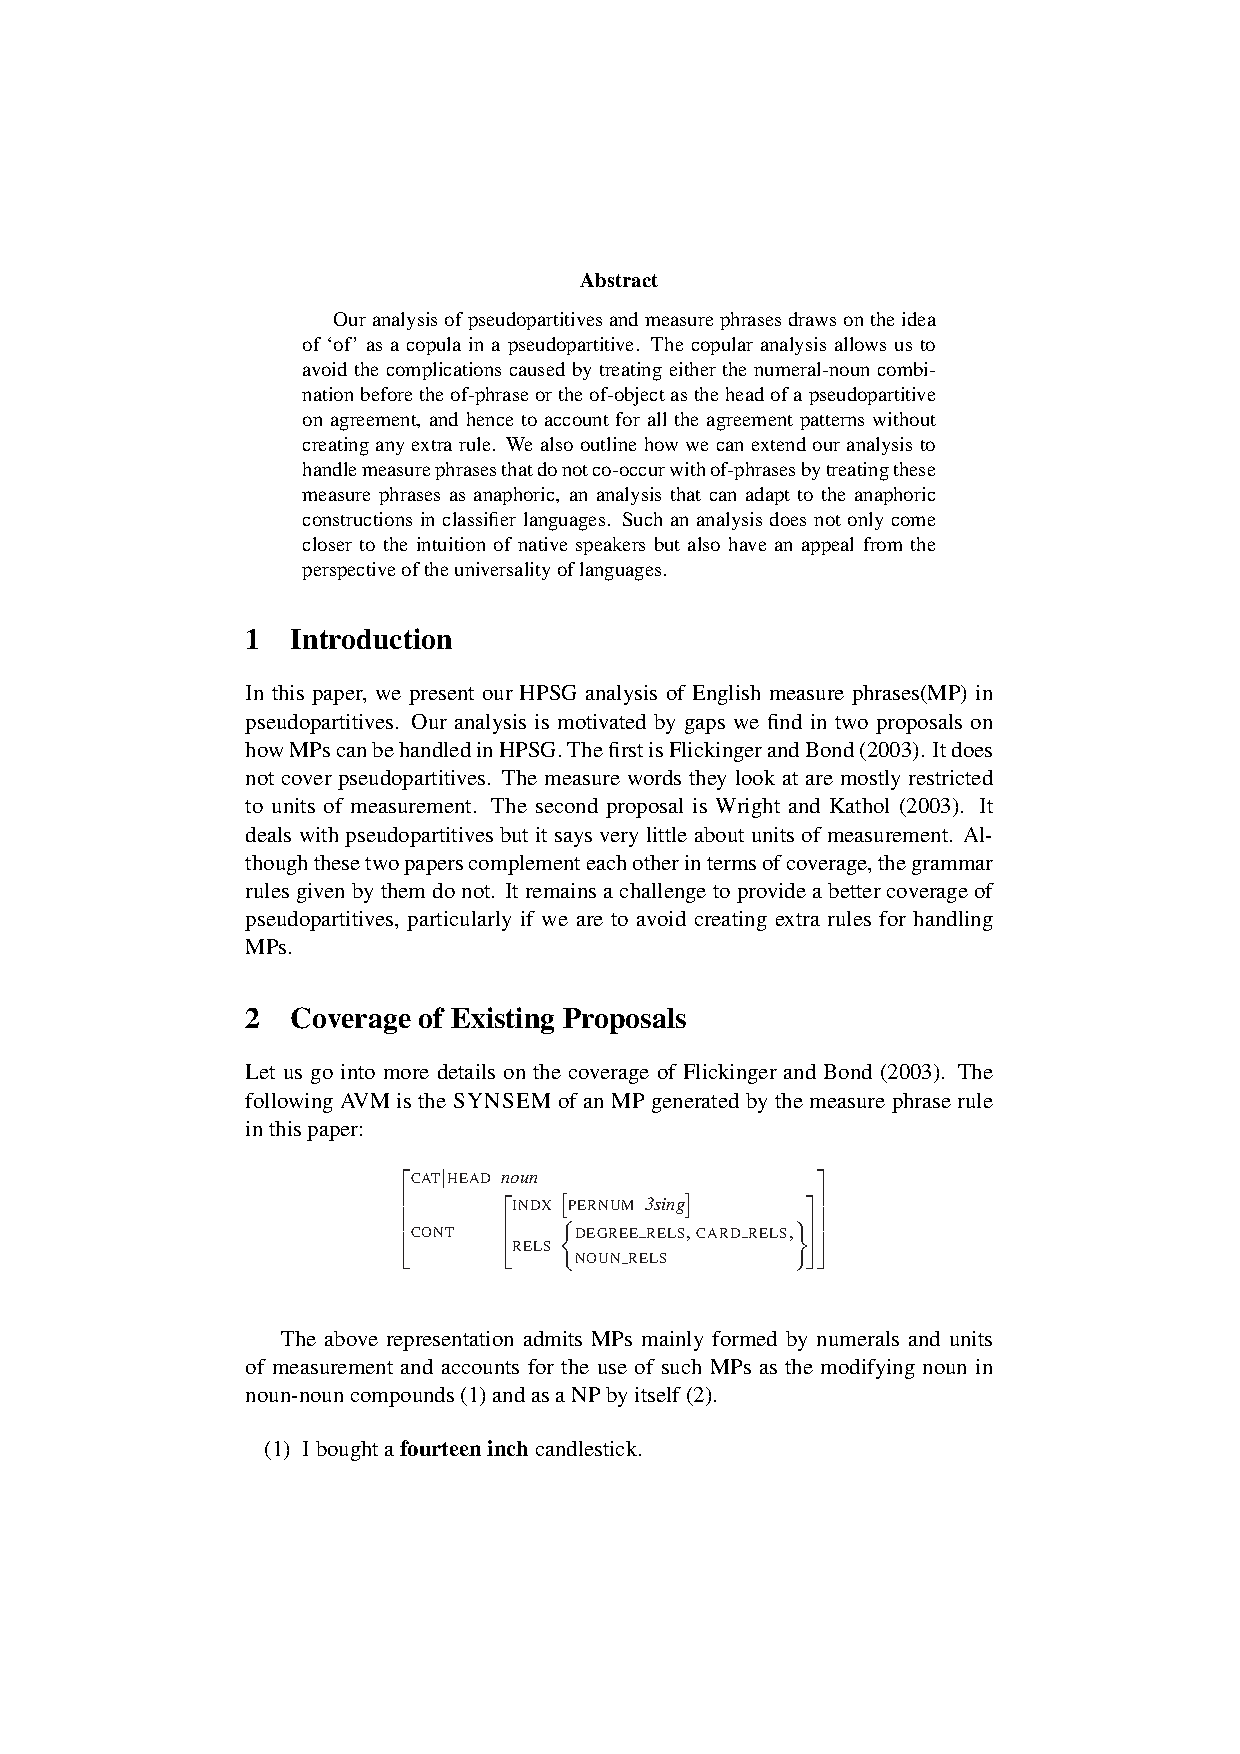
\includepdf[pages=-,pagecommand=\thispagestyle{plain}]{Includes/tam-sato.pdf}
        \setcounter{page}{234}
        \phantomsection
        \addcontentsline{toc}{section}{Jesse Tseng: The representation of syllable structure in HPSG}
\thispagestyle{empty}

\begin{center}
  {\huge\bfseries The representation of syllable structure in HPSG\par}

  \bigskip

~\\
\begingroup
\setlength{\leftskip}{0pt plus 1fill}
\setlength{\rightskip}{0pt plus 1fill}
\setlength{\parindent}{0pt}
\setlength{\parfillskip}{0pt}
  \formatauthor{Jesse Tseng}{\begin{tabular}{@{}c@{}}CNRS\end{tabular}}

\par\endgroup

  \vspace*{8ex}

  Proceedings of the 15th International Conference on\par Head-Driven Phrase Structure Grammar

  \bigskip

  National Institute of Information and Communications Technology, Keihanna

  \medskip

  Stefan Müller (Editor)

  \medskip

  2008

  \medskip

  CSLI Publications

  \medskip

  pages 234--252

  \medskip

  \url{http://csli-publications.stanford.edu/HPSG/2008}
\end{center}
\vfill

\noindent



\vfill
\noindent
% APA Style
Tseng, Jesse. 2008. The representation of syllable structure in HPSG. In Müller, Stefan (Ed.), \emph{{Proceedings of the 15th International Conference on Head-Driven Phrase Structure Grammar, National Institute of Information and Communications Technology, Keihanna}}, 234--252. Stanford,
CA: CSLI Publications. \hfill\href{http://creativecommons.org/licenses/by/4.0/}{\includegraphics[height=.75em]{Includes/ccby.eps}}

\newpage
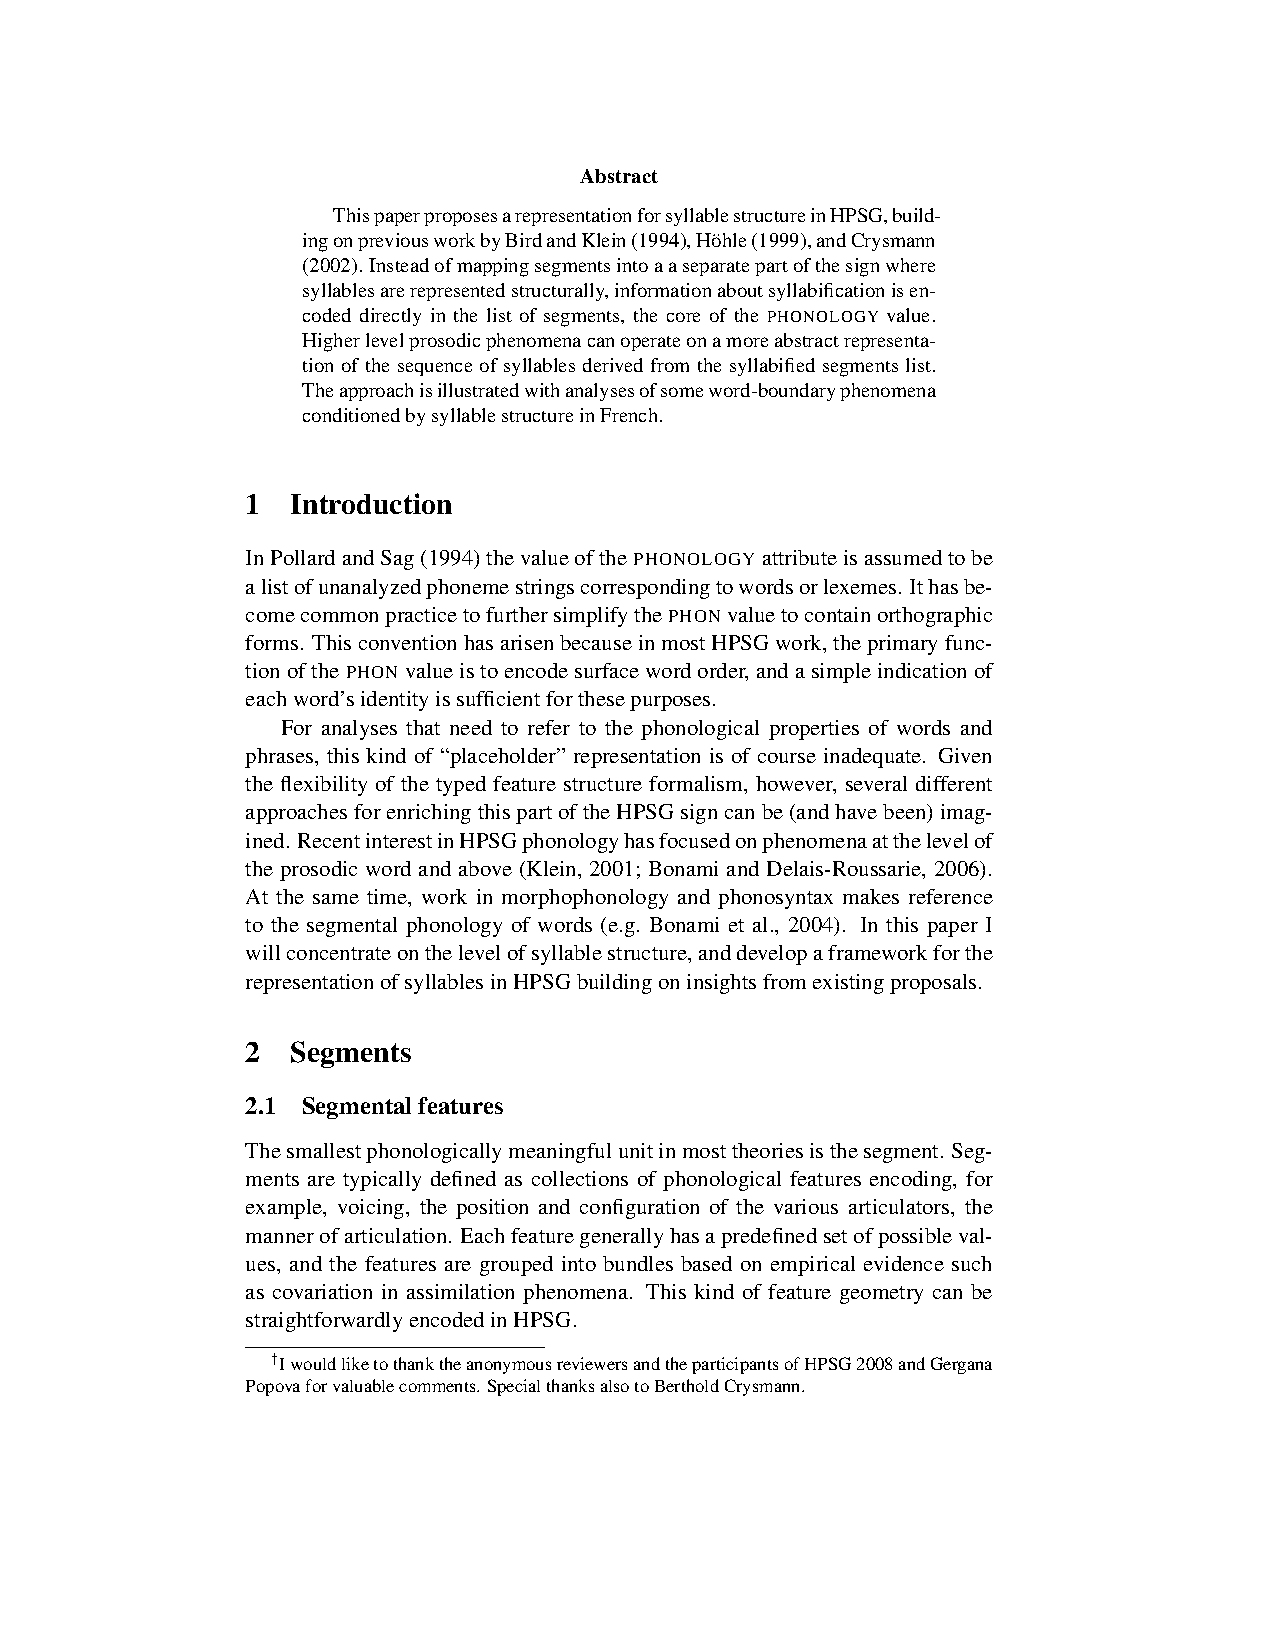
\includepdf[pages=-,pagecommand=\thispagestyle{plain}]{Includes/tseng.pdf}
        \setcounter{page}{253}
        \phantomsection
        \addcontentsline{toc}{section}{Frank Van Eynde: Predicate Complements}
\thispagestyle{empty}

\begin{center}
  {\huge\bfseries Predicate Complements\par}

  \bigskip

~\\
\begingroup
\setlength{\leftskip}{0pt plus 1fill}
\setlength{\rightskip}{0pt plus 1fill}
\setlength{\parindent}{0pt}
\setlength{\parfillskip}{0pt}
  \formatauthor{Frank Van Eynde}{\begin{tabular}{@{}c@{}}University of Leuven\end{tabular}}

\par\endgroup

  \vspace*{8ex}

  Proceedings of the 15th International Conference on\par Head-Driven Phrase Structure Grammar

  \bigskip

  National Institute of Information and Communications Technology, Keihanna

  \medskip

  Stefan Müller (Editor)

  \medskip

  2008

  \medskip

  CSLI Publications

  \medskip

  pages 253--273

  \medskip

  \url{http://csli-publications.stanford.edu/HPSG/2008}
\end{center}
\vfill

\noindent



\vfill
\noindent
% APA Style
Van Eynde, Frank. 2008. Predicate Complements. In Müller, Stefan (Ed.), \emph{{Proceedings of the 15th International Conference on Head-Driven Phrase Structure Grammar, National Institute of Information and Communications Technology, Keihanna}}, 253--273. Stanford,
CA: CSLI Publications. \hfill\href{http://creativecommons.org/licenses/by/4.0/}{\includegraphics[height=.75em]{Includes/ccby.eps}}

\newpage
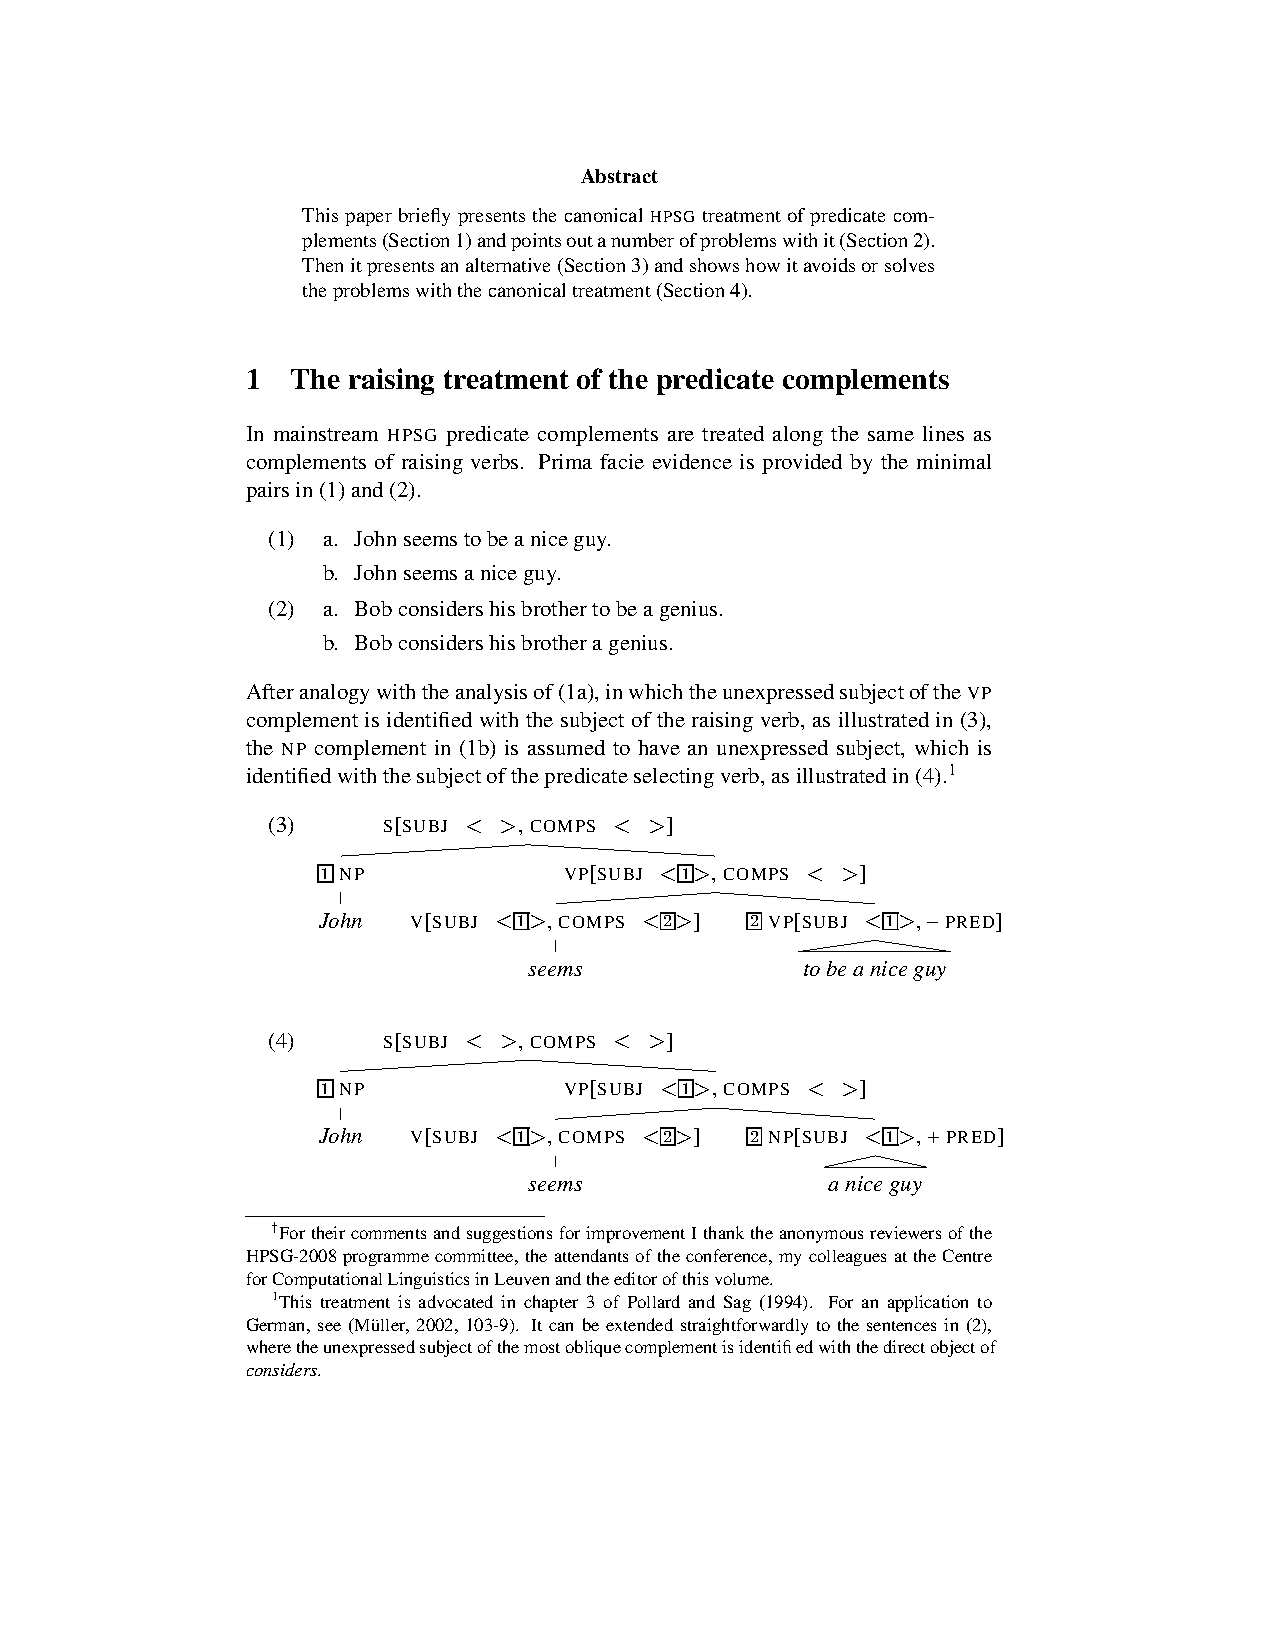
\includepdf[pages=-,pagecommand=\thispagestyle{plain}]{Includes/vaneynde.pdf}
        \setcounter{page}{274}
        \phantomsection
        \addcontentsline{toc}{section}{Stephen Wechsler: Dualist Syntax}
\thispagestyle{empty}

\begin{center}
  {\huge\bfseries Dualist Syntax\par}

  \bigskip

~\\
\begingroup
\setlength{\leftskip}{0pt plus 1fill}
\setlength{\rightskip}{0pt plus 1fill}
\setlength{\parindent}{0pt}
\setlength{\parfillskip}{0pt}
  \formatauthor{Stephen Wechsler}{\begin{tabular}{@{}c@{}}University of Texas at Austin\end{tabular}}

\par\endgroup

  \vspace*{8ex}

  Proceedings of the 15th International Conference on\par Head-Driven Phrase Structure Grammar

  \bigskip

  National Institute of Information and Communications Technology, Keihanna

  \medskip

  Stefan Müller (Editor)

  \medskip

  2008

  \medskip

  CSLI Publications

  \medskip

  pages 274--293

  \medskip

  \url{http://csli-publications.stanford.edu/HPSG/2008}
\end{center}
\vfill

\noindent



\vfill
\noindent
% APA Style
Wechsler, Stephen. 2008. Dualist Syntax. In Müller, Stefan (Ed.), \emph{{Proceedings of the 15th International Conference on Head-Driven Phrase Structure Grammar, National Institute of Information and Communications Technology, Keihanna}}, 274--293. Stanford,
CA: CSLI Publications. \hfill\href{http://creativecommons.org/licenses/by/4.0/}{\includegraphics[height=.75em]{Includes/ccby.eps}}

\newpage
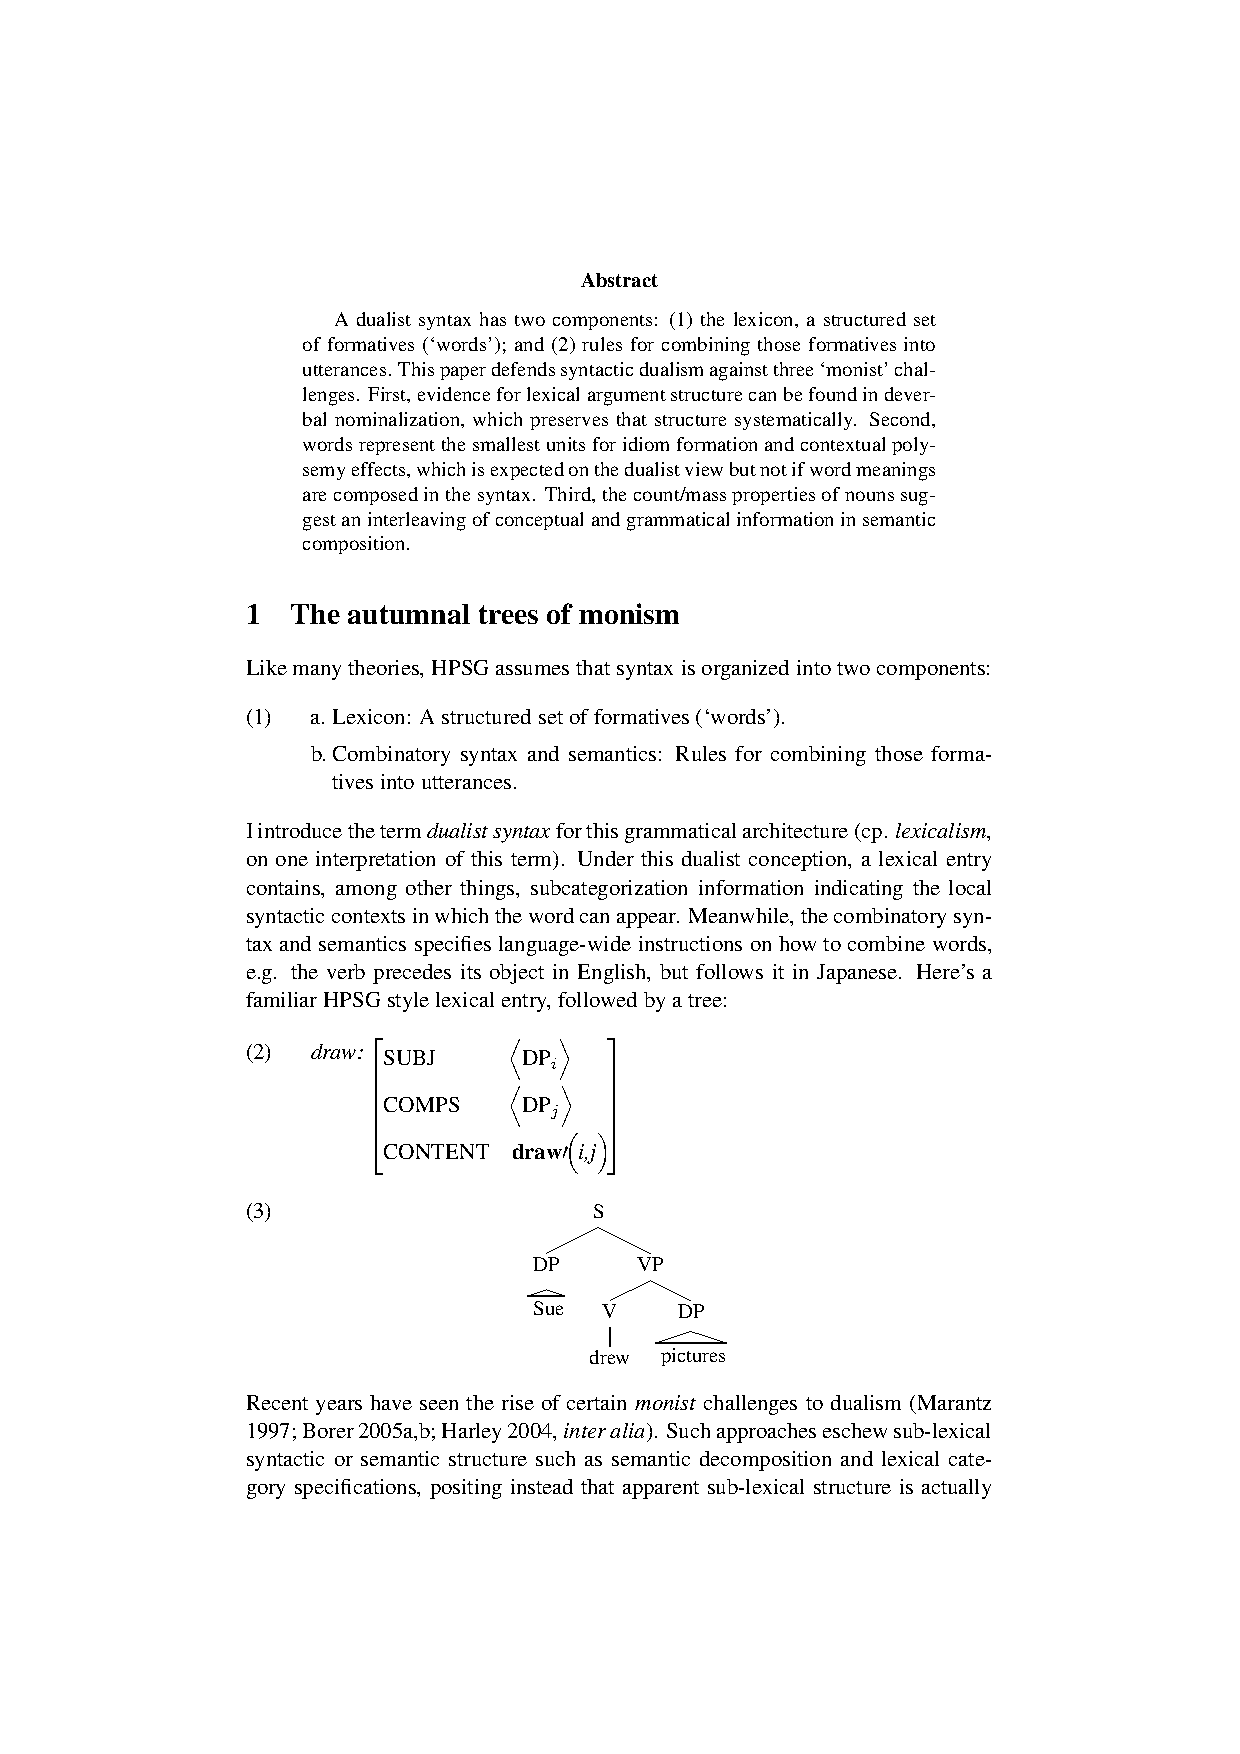
\includepdf[pages=-,pagecommand=\thispagestyle{plain}]{Includes/wechsler.pdf}
        \setcounter{page}{294}
        \phantomsection
        \addcontentsline{toc}{section}{Eun-Jung Yoo: Transparent Free Relatives in English}
\thispagestyle{empty}

\begin{center}
  {\huge\bfseries Transparent Free Relatives in English\par}

  \bigskip

~\\
\begingroup
\setlength{\leftskip}{0pt plus 1fill}
\setlength{\rightskip}{0pt plus 1fill}
\setlength{\parindent}{0pt}
\setlength{\parfillskip}{0pt}
  \formatauthor{Eun-Jung Yoo}{\begin{tabular}{@{}c@{}}Seoul National University\end{tabular}}

\par\endgroup

  \vspace*{8ex}

  Proceedings of the 15th International Conference on\par Head-Driven Phrase Structure Grammar

  \bigskip

  National Institute of Information and Communications Technology, Keihanna

  \medskip

  Stefan Müller (Editor)

  \medskip

  2008

  \medskip

  CSLI Publications

  \medskip

  pages 294--304

  \medskip

  \url{http://csli-publications.stanford.edu/HPSG/2008}
\end{center}
\vfill

\noindent



\vfill
\noindent
% APA Style
Yoo, Eun-Jung. 2008. Transparent Free Relatives in English. In Müller, Stefan (Ed.), \emph{{Proceedings of the 15th International Conference on Head-Driven Phrase Structure Grammar, National Institute of Information and Communications Technology, Keihanna}}, 294--304. Stanford,
CA: CSLI Publications. \hfill\href{http://creativecommons.org/licenses/by/4.0/}{\includegraphics[height=.75em]{Includes/ccby.eps}}

\newpage
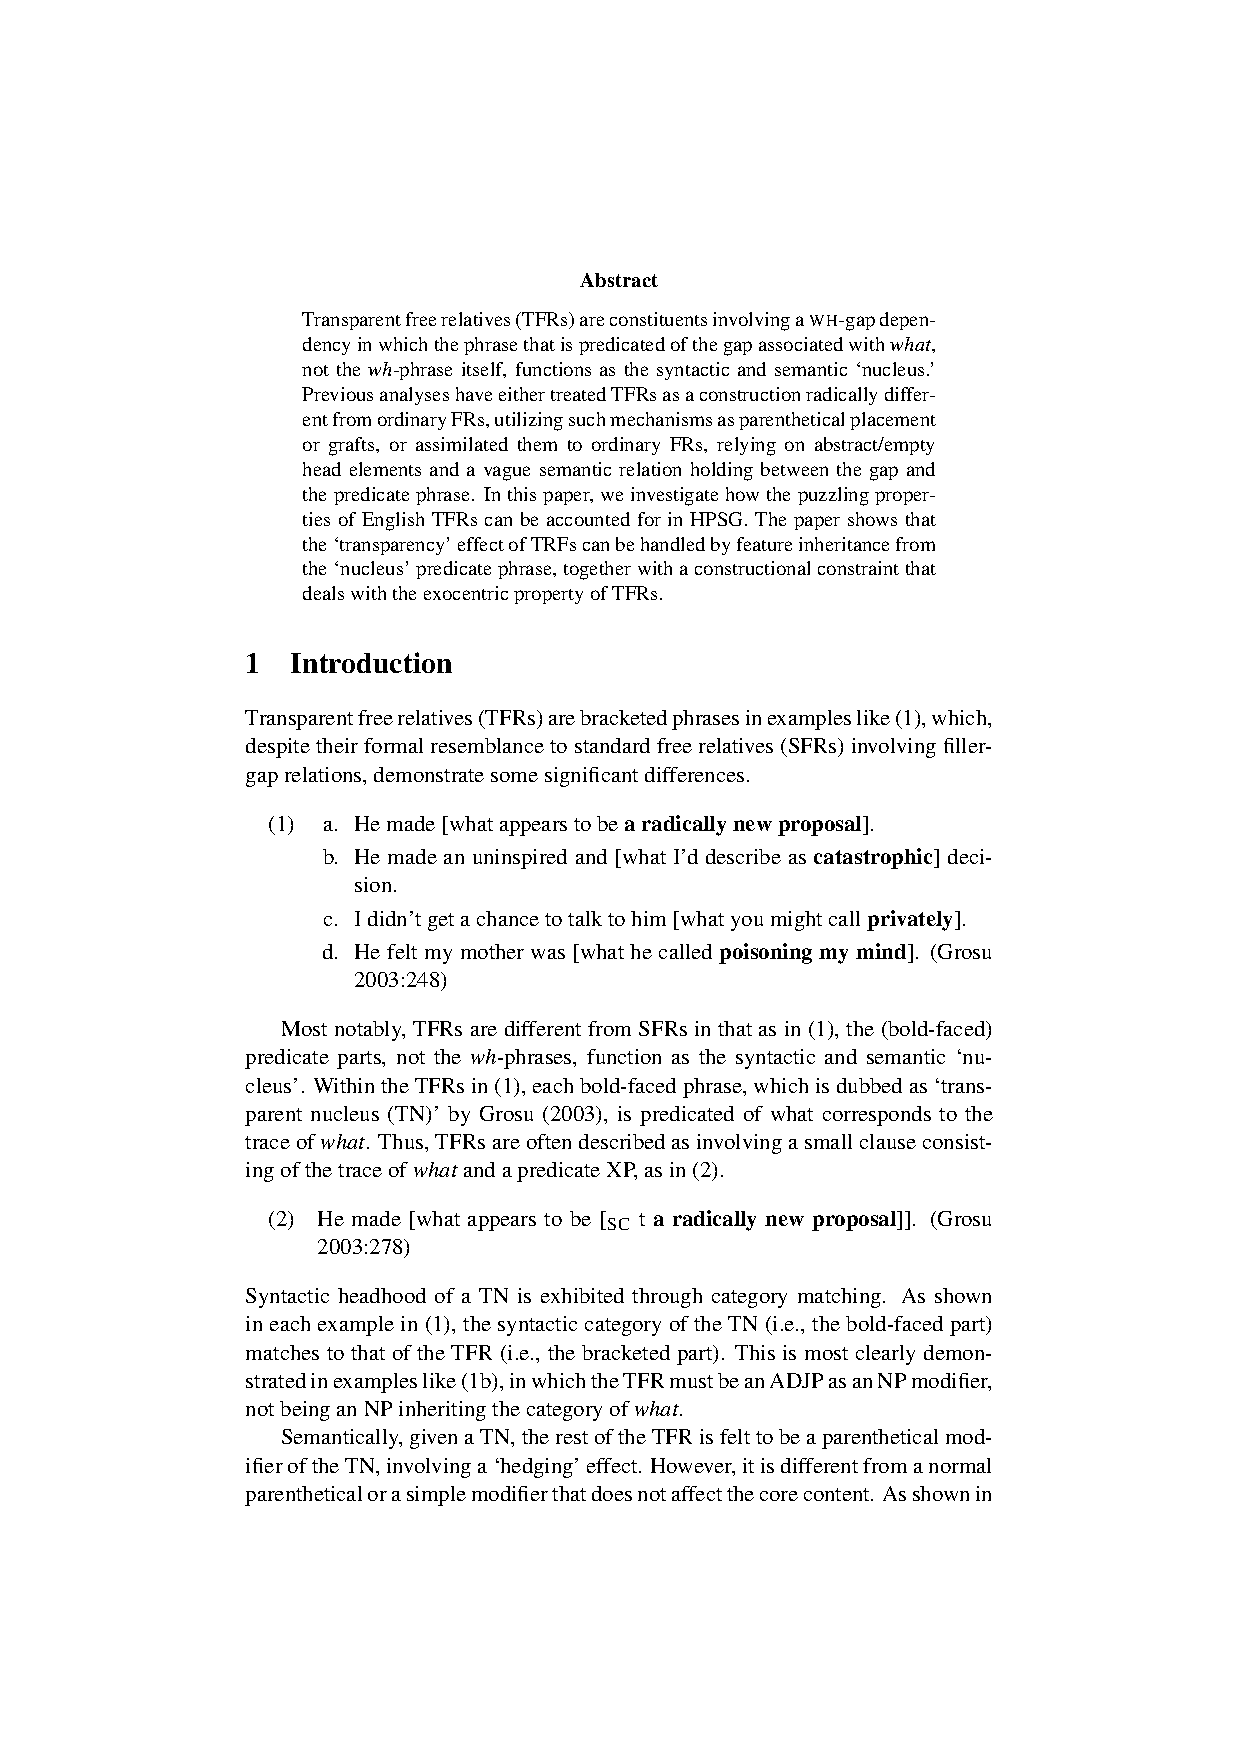
\includepdf[pages=-,pagecommand=\thispagestyle{plain}]{Includes/yoo.pdf}
\part{Contributions to the Workshop}
\thispagestyle{empty}
\newpage
        \setcounter{page}{306}
        \phantomsection
        \addcontentsline{toc}{section}{Anne Abeill{\'e}, Dani\`{e}le Godard, Fr{\'e}d{\'e}ric Sabio: Two types of NP preposing in French}
\thispagestyle{empty}

\begin{center}
  {\huge\bfseries Two types of NP preposing in French\par}

  \bigskip

~\\
\begingroup
\setlength{\leftskip}{0pt plus 1fill}
\setlength{\rightskip}{0pt plus 1fill}
\setlength{\parindent}{0pt}
\setlength{\parfillskip}{0pt}
  \formatauthor{Anne Abeillé}{\begin{tabular}{@{}c@{}}University of Paris 7\end{tabular}}
\formatauthor{Danièle Godard}{\begin{tabular}{@{}c@{}}CNRS, France\end{tabular}}
\formatauthor{Frédéric Sabio}{\begin{tabular}{@{}c@{}}University of Paris 7\end{tabular}}

\par\endgroup

  \vspace*{8ex}

  Proceedings of the 15th International Conference on\par Head-Driven Phrase Structure Grammar

  \bigskip

  National Institute of Information and Communications Technology, Keihanna

  \medskip

  Stefan Müller (Editor)

  \medskip

  2008

  \medskip

  CSLI Publications

  \medskip

  pages 306--324

  \medskip

  \url{http://csli-publications.stanford.edu/HPSG/2008}
\end{center}
\vfill

\noindent



\vfill
\noindent
% APA Style
Abeillé, Anne, Godard,  Danièle, \& Sabio, Frédéric. 2008. Two types of NP preposing in French. In Müller, Stefan (Ed.), \emph{{Proceedings of the 15th International Conference on Head-Driven Phrase Structure Grammar, National Institute of Information and Communications Technology, Keihanna}}, 306--324. Stanford,
CA: CSLI Publications. \hfill\href{http://creativecommons.org/licenses/by/4.0/}{\includegraphics[height=.75em]{Includes/ccby.eps}}

\newpage
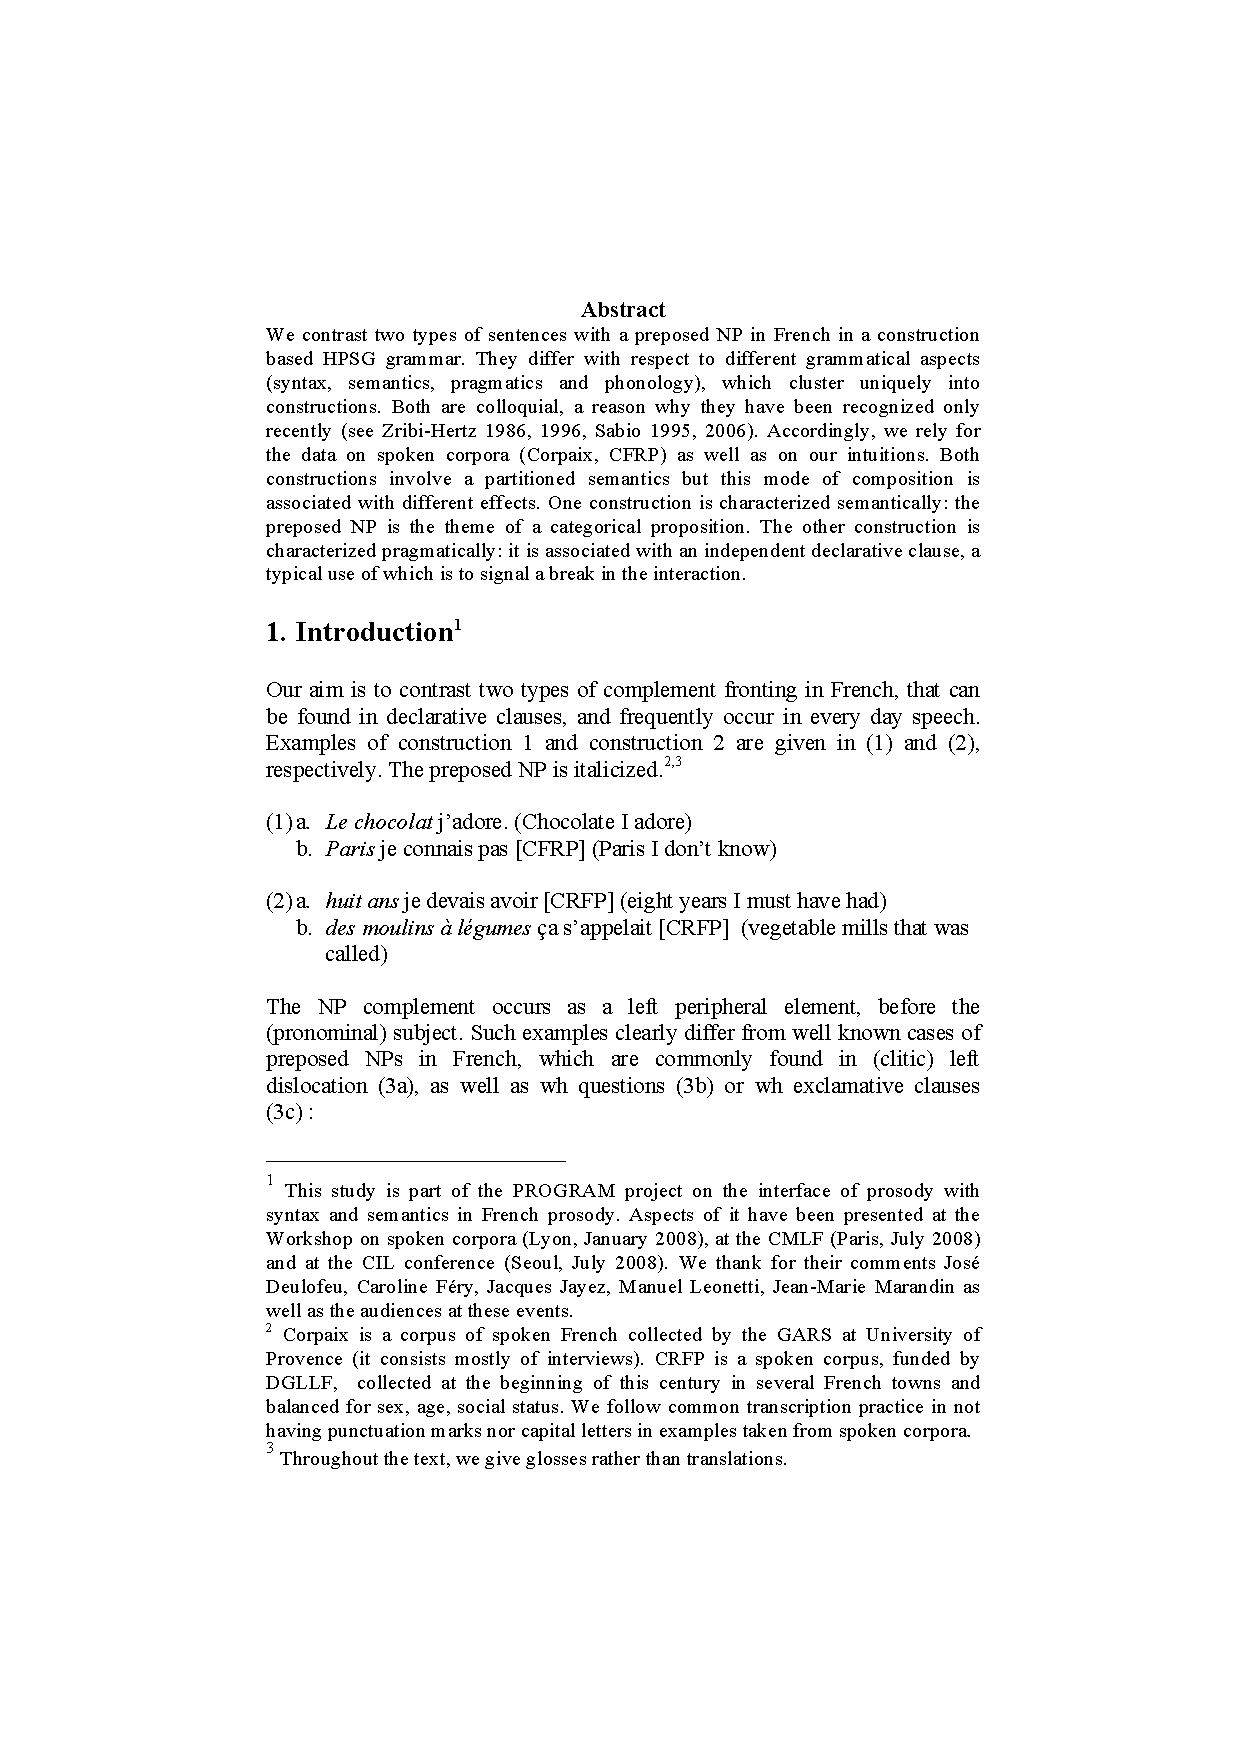
\includepdf[pages=-,pagecommand=\thispagestyle{plain}]{Includes/ags.pdf}
        \setcounter{page}{325}
        \phantomsection
        \addcontentsline{toc}{section}{Doug Arnold, Robert D Borsley: Non-restrictive Relative Clauses, Ellipsis and Anaphora}
\thispagestyle{empty}

\begin{center}
  {\huge\bfseries Non-restrictive Relative Clauses, Ellipsis and Anaphora\par}

  \bigskip

~\\
\begingroup
\setlength{\leftskip}{0pt plus 1fill}
\setlength{\rightskip}{0pt plus 1fill}
\setlength{\parindent}{0pt}
\setlength{\parfillskip}{0pt}
  \formatauthor{Doug Arnold}{\begin{tabular}{@{}c@{}}University of Essex\end{tabular}}
\formatauthor{Robert D Borsley}{\begin{tabular}{@{}c@{}}University of Essex\end{tabular}}

\par\endgroup

  \vspace*{8ex}

  Proceedings of the 15th International Conference on\par Head-Driven Phrase Structure Grammar

  \bigskip

  National Institute of Information and Communications Technology, Keihanna

  \medskip

  Stefan Müller (Editor)

  \medskip

  2008

  \medskip

  CSLI Publications

  \medskip

  pages 325--345

  \medskip

  \url{http://csli-publications.stanford.edu/HPSG/2008}
\end{center}
\vfill

\noindent



\vfill
\noindent
% APA Style
Arnold, Doug, \& Borsley, Robert D. 2008. Non-restrictive Relative Clauses, Ellipsis and Anaphora. In Müller, Stefan (Ed.), \emph{{Proceedings of the 15th International Conference on Head-Driven Phrase Structure Grammar, National Institute of Information and Communications Technology, Keihanna}}, 325--345. Stanford,
CA: CSLI Publications. \hfill\href{http://creativecommons.org/licenses/by/4.0/}{\includegraphics[height=.75em]{Includes/ccby.eps}}

\newpage
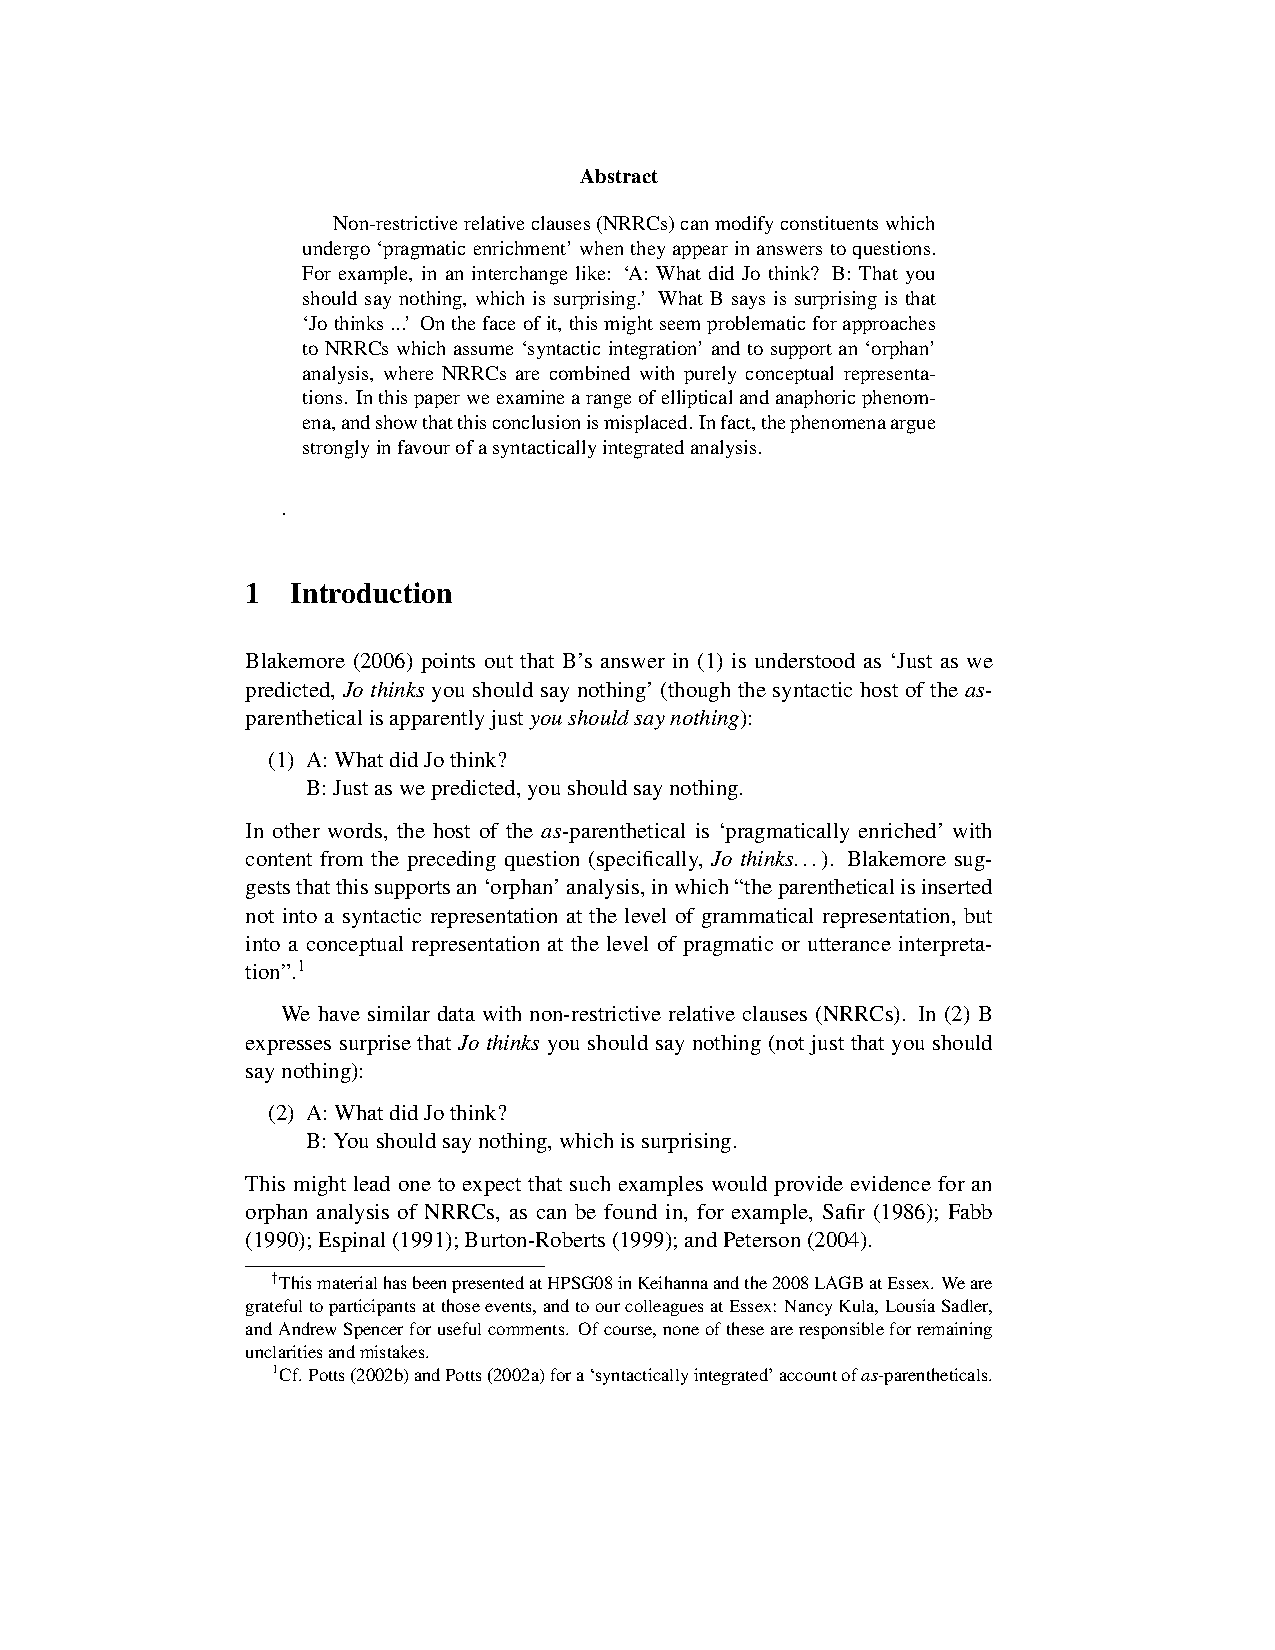
\includepdf[pages=-,pagecommand=\thispagestyle{plain}]{Includes/arnold-borsley.pdf}
        \setcounter{page}{346}
        \phantomsection
        \addcontentsline{toc}{section}{Felix Bildhauer: Clitic left dislocation and focus projection in Spanish}
\thispagestyle{empty}

\begin{center}
  {\huge\bfseries Clitic left dislocation and focus projection in Spanish\par}

  \bigskip

~\\
\begingroup
\setlength{\leftskip}{0pt plus 1fill}
\setlength{\rightskip}{0pt plus 1fill}
\setlength{\parindent}{0pt}
\setlength{\parfillskip}{0pt}
  \formatauthor{Felix Bildhauer}{\begin{tabular}{@{}c@{}}Freie Universität Berlin\end{tabular}}

\par\endgroup

  \vspace*{8ex}

  Proceedings of the 15th International Conference on\par Head-Driven Phrase Structure Grammar

  \bigskip

  National Institute of Information and Communications Technology, Keihanna

  \medskip

  Stefan Müller (Editor)

  \medskip

  2008

  \medskip

  CSLI Publications

  \medskip

  pages 346--357

  \medskip

  \url{http://csli-publications.stanford.edu/HPSG/2008}
\end{center}
\vfill

\noindent



\vfill
\noindent
% APA Style
Bildhauer, Felix. 2008. Clitic left dislocation and focus projection in Spanish. In Müller, Stefan (Ed.), \emph{{Proceedings of the 15th International Conference on Head-Driven Phrase Structure Grammar, National Institute of Information and Communications Technology, Keihanna}}, 346--357. Stanford,
CA: CSLI Publications. \hfill\href{http://creativecommons.org/licenses/by/4.0/}{\includegraphics[height=.75em]{Includes/ccby.eps}}

\newpage
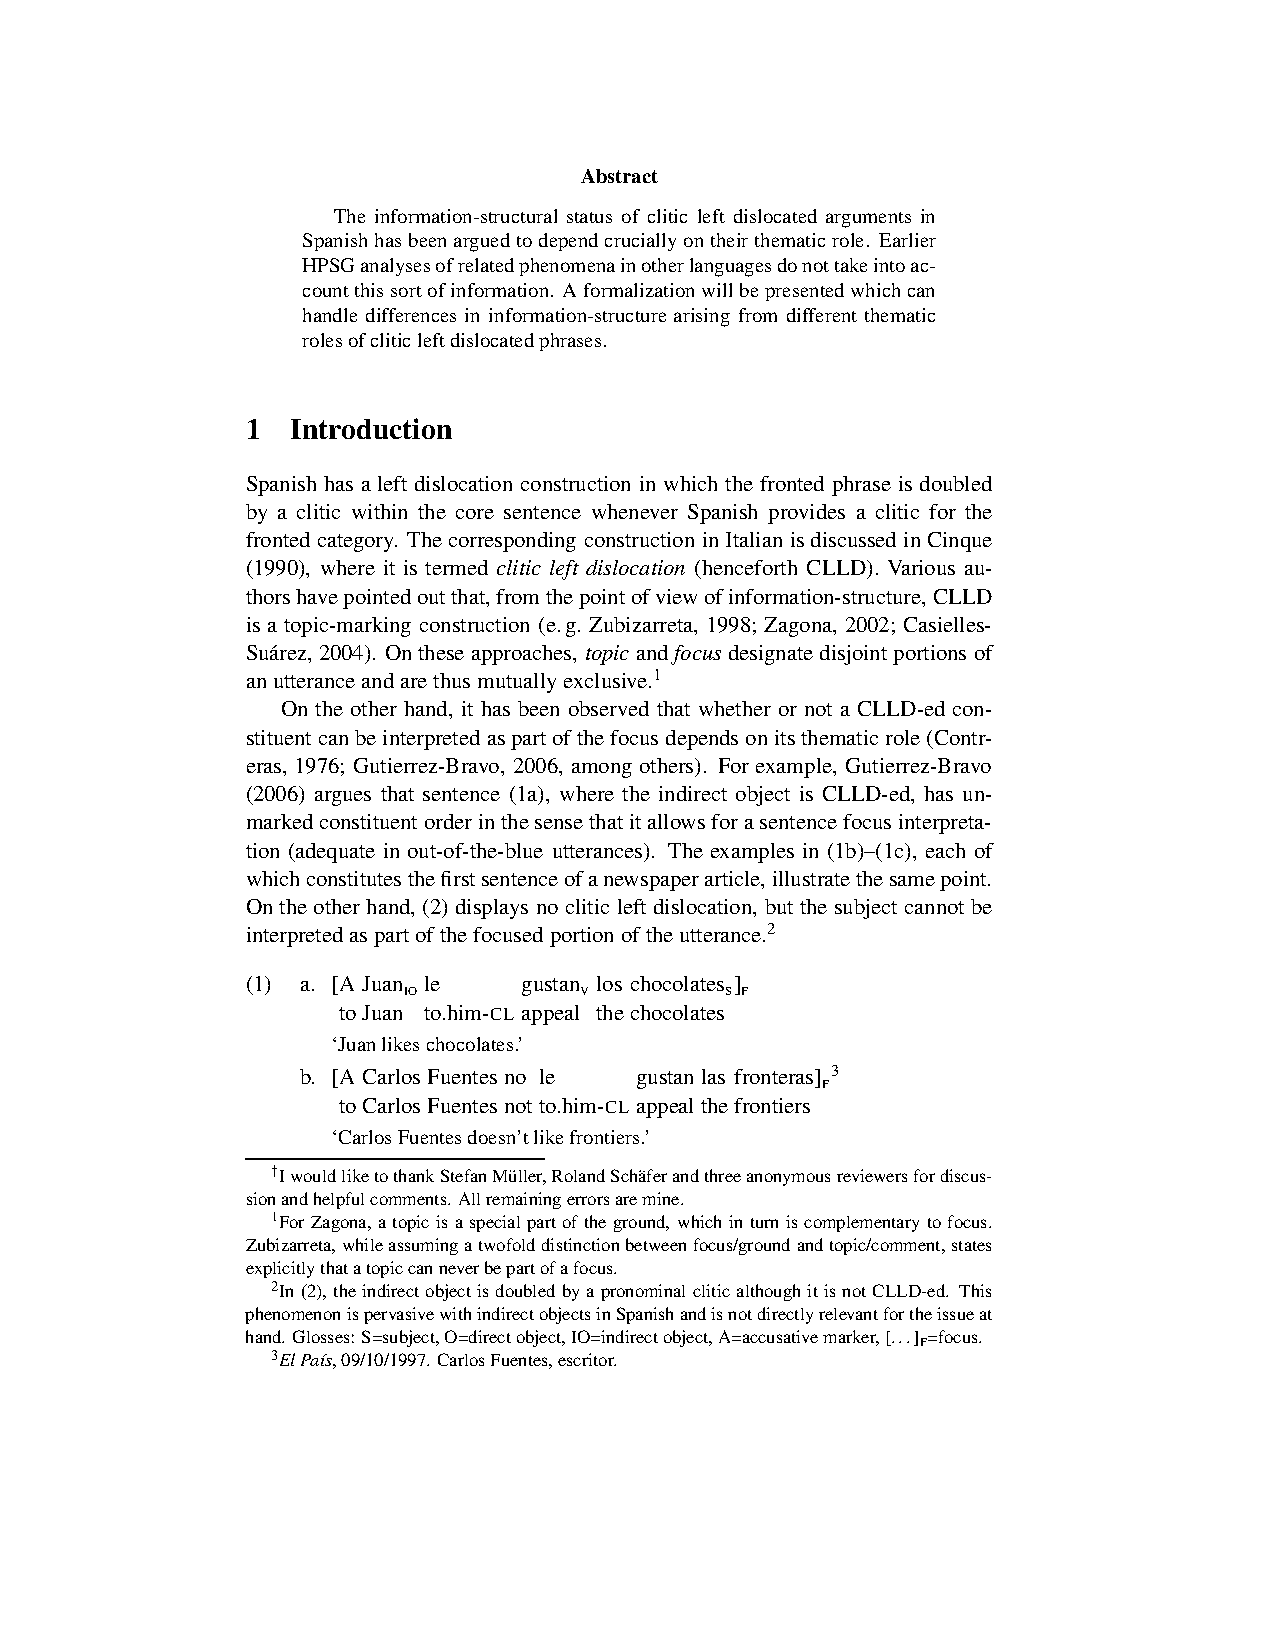
\includepdf[pages=-,pagecommand=\thispagestyle{plain}]{Includes/bildhauer.pdf}
        \setcounter{page}{358}
        \phantomsection
        \addcontentsline{toc}{section}{Olivier Bonami, Dani\`{e}le Godard: On the syntax of direct quotation in French}
\thispagestyle{empty}

\begin{center}
  {\huge\bfseries On the syntax of direct quotation in French\par}

  \bigskip

~\\
\begingroup
\setlength{\leftskip}{0pt plus 1fill}
\setlength{\rightskip}{0pt plus 1fill}
\setlength{\parindent}{0pt}
\setlength{\parfillskip}{0pt}
  \formatauthor{Olivier Bonami}{\begin{tabular}{@{}c@{}}Université Paris-Sorbonne\end{tabular}}
\formatauthor{Danièle Godard}{\begin{tabular}{@{}c@{}}LLF\end{tabular}}

\par\endgroup

  \vspace*{8ex}

  Proceedings of the 15th International Conference on\par Head-Driven Phrase Structure Grammar

  \bigskip

  National Institute of Information and Communications Technology, Keihanna

  \medskip

  Stefan Müller (Editor)

  \medskip

  2008

  \medskip

  CSLI Publications

  \medskip

  pages 358--377

  \medskip

  \url{http://csli-publications.stanford.edu/HPSG/2008}
\end{center}
\vfill

\noindent



\vfill
\noindent
% APA Style
Bonami, Olivier, \& Godard, Danièle. 2008. On the syntax of direct quotation in French. In Müller, Stefan (Ed.), \emph{{Proceedings of the 15th International Conference on Head-Driven Phrase Structure Grammar, National Institute of Information and Communications Technology, Keihanna}}, 358--377. Stanford,
CA: CSLI Publications. \hfill\href{http://creativecommons.org/licenses/by/4.0/}{\includegraphics[height=.75em]{Includes/ccby.eps}}

\newpage
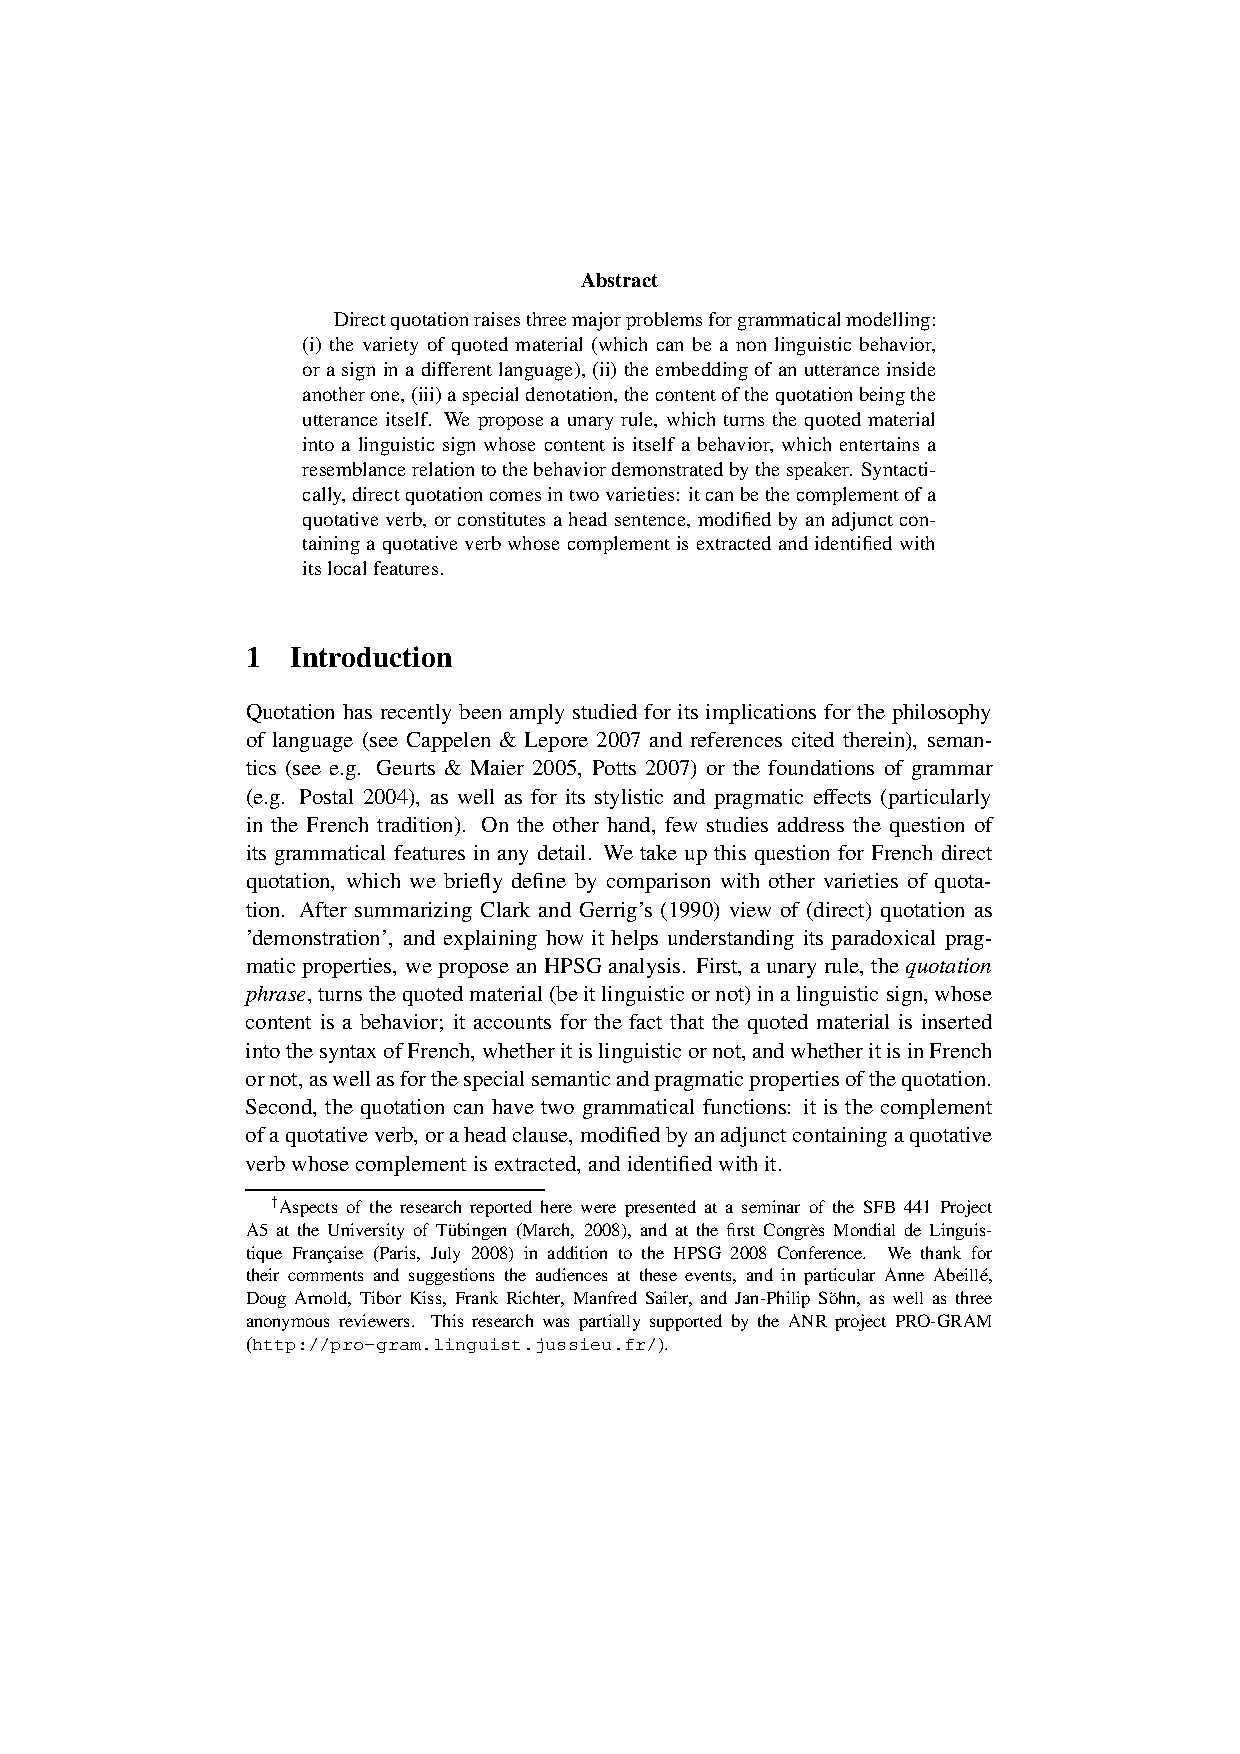
\includepdf[pages=-,pagecommand=\thispagestyle{plain}]{Includes/bonami-godard.pdf}
        \setcounter{page}{378}
        \phantomsection
        \addcontentsline{toc}{section}{Fabiola Henri, Anne Abeill{\'e}: Verb Form Alternations in Mauritian}
\thispagestyle{empty}

\begin{center}
  {\huge\bfseries Verb Form Alternations in Mauritian\par}

  \bigskip

~\\
\begingroup
\setlength{\leftskip}{0pt plus 1fill}
\setlength{\rightskip}{0pt plus 1fill}
\setlength{\parindent}{0pt}
\setlength{\parfillskip}{0pt}
  \formatauthor{Fabiola Henri}{\begin{tabular}{@{}c@{}}Université Paris-Sorbonne\end{tabular}}
\formatauthor{Anne Abeillé}{\begin{tabular}{@{}c@{}}LLF\end{tabular}}

\par\endgroup

  \vspace*{8ex}

  Proceedings of the 15th International Conference on\par Head-Driven Phrase Structure Grammar

  \bigskip

  National Institute of Information and Communications Technology, Keihanna

  \medskip

  Stefan Müller (Editor)

  \medskip

  2008

  \medskip

  CSLI Publications

  \medskip

  pages 378--398

  \medskip

  \url{http://csli-publications.stanford.edu/HPSG/2008}
\end{center}
\vfill

\noindent



\vfill
\noindent
% APA Style
Henri, Fabiola, \& Abeillé, Anne. 2008. Verb Form Alternations in Mauritian. In Müller, Stefan (Ed.), \emph{{Proceedings of the 15th International Conference on Head-Driven Phrase Structure Grammar, National Institute of Information and Communications Technology, Keihanna}}, 378--398. Stanford,
CA: CSLI Publications. \hfill\href{http://creativecommons.org/licenses/by/4.0/}{\includegraphics[height=.75em]{Includes/ccby.eps}}

\newpage
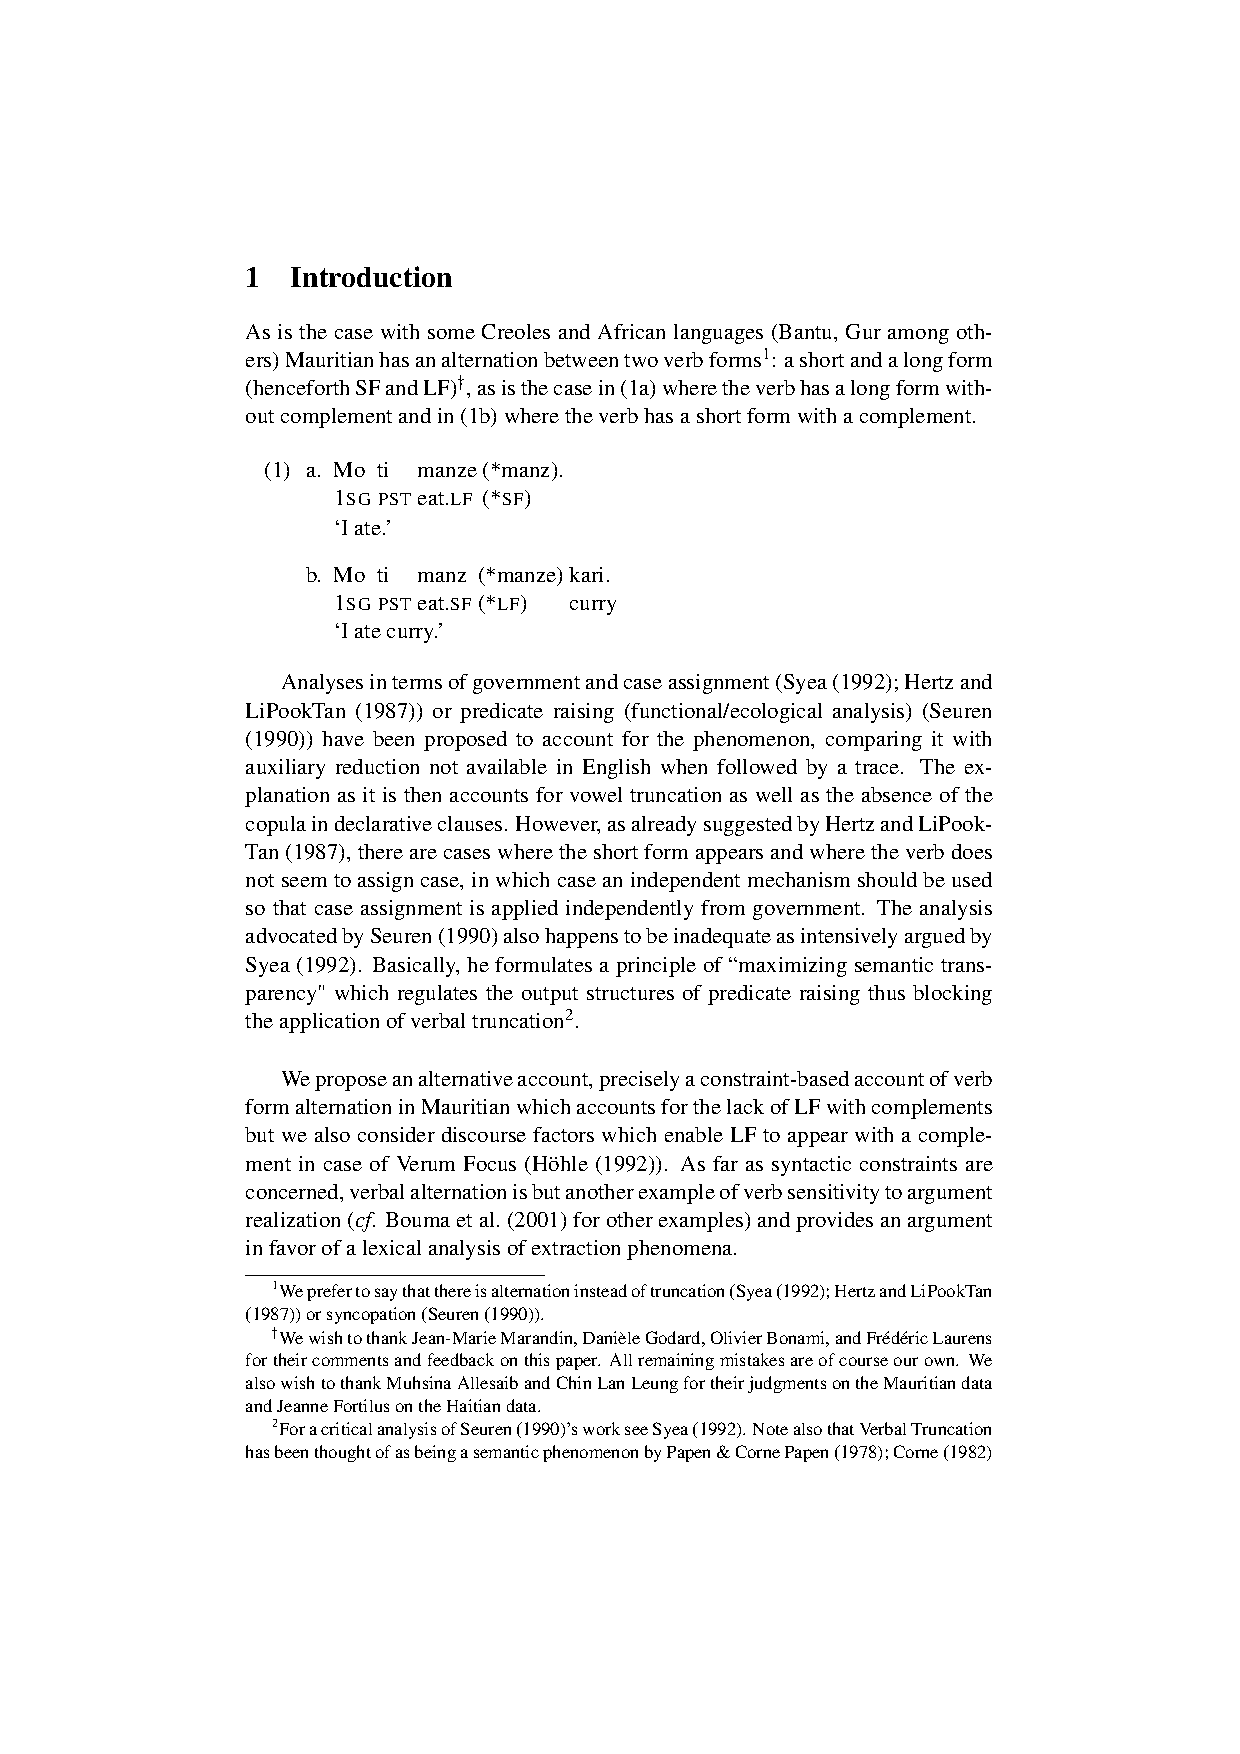
\includepdf[pages=-,pagecommand=\thispagestyle{plain}]{Includes/henri-abeille.pdf}
        \setcounter{page}{399}
        \phantomsection
        \addcontentsline{toc}{section}{Mutsumi Imai: Children's use of argument structure, meta-knowledge of the lexicon, and extra-linguistic contextual cues in inferring meanings of novel verbs}
\thispagestyle{empty}

\begin{center}
  {\huge\bfseries Children's use of argument structure, meta-knowledge of the lexicon, and extra-linguistic contextual cues in inferring meanings of novel verbs\par}

  \bigskip

~\\
\begingroup
\setlength{\leftskip}{0pt plus 1fill}
\setlength{\rightskip}{0pt plus 1fill}
\setlength{\parindent}{0pt}
\setlength{\parfillskip}{0pt}
  \formatauthor{Mutsumi Imai}{\begin{tabular}{@{}c@{}}Keio University\end{tabular}}

\par\endgroup

  \vspace*{8ex}

  Proceedings of the 15th International Conference on\par Head-Driven Phrase Structure Grammar

  \bigskip

  National Institute of Information and Communications Technology, Keihanna

  \medskip

  Stefan Müller (Editor)

  \medskip

  2008

  \medskip

  CSLI Publications

  \medskip

  pages 399--416

  \medskip

  \url{http://csli-publications.stanford.edu/HPSG/2008}
\end{center}
\vfill

\noindent



\vfill
\noindent
% APA Style
Imai, Mutsumi. 2008. Children's use of argument structure, meta-knowledge of the lexicon, and extra-linguistic contextual cues in inferring meanings of novel verbs. In Müller, Stefan (Ed.), \emph{{Proceedings of the 15th International Conference on Head-Driven Phrase Structure Grammar, National Institute of Information and Communications Technology, Keihanna}}, 399--416. Stanford,
CA: CSLI Publications. \hfill\href{http://creativecommons.org/licenses/by/4.0/}{\includegraphics[height=.75em]{Includes/ccby.eps}}

\newpage
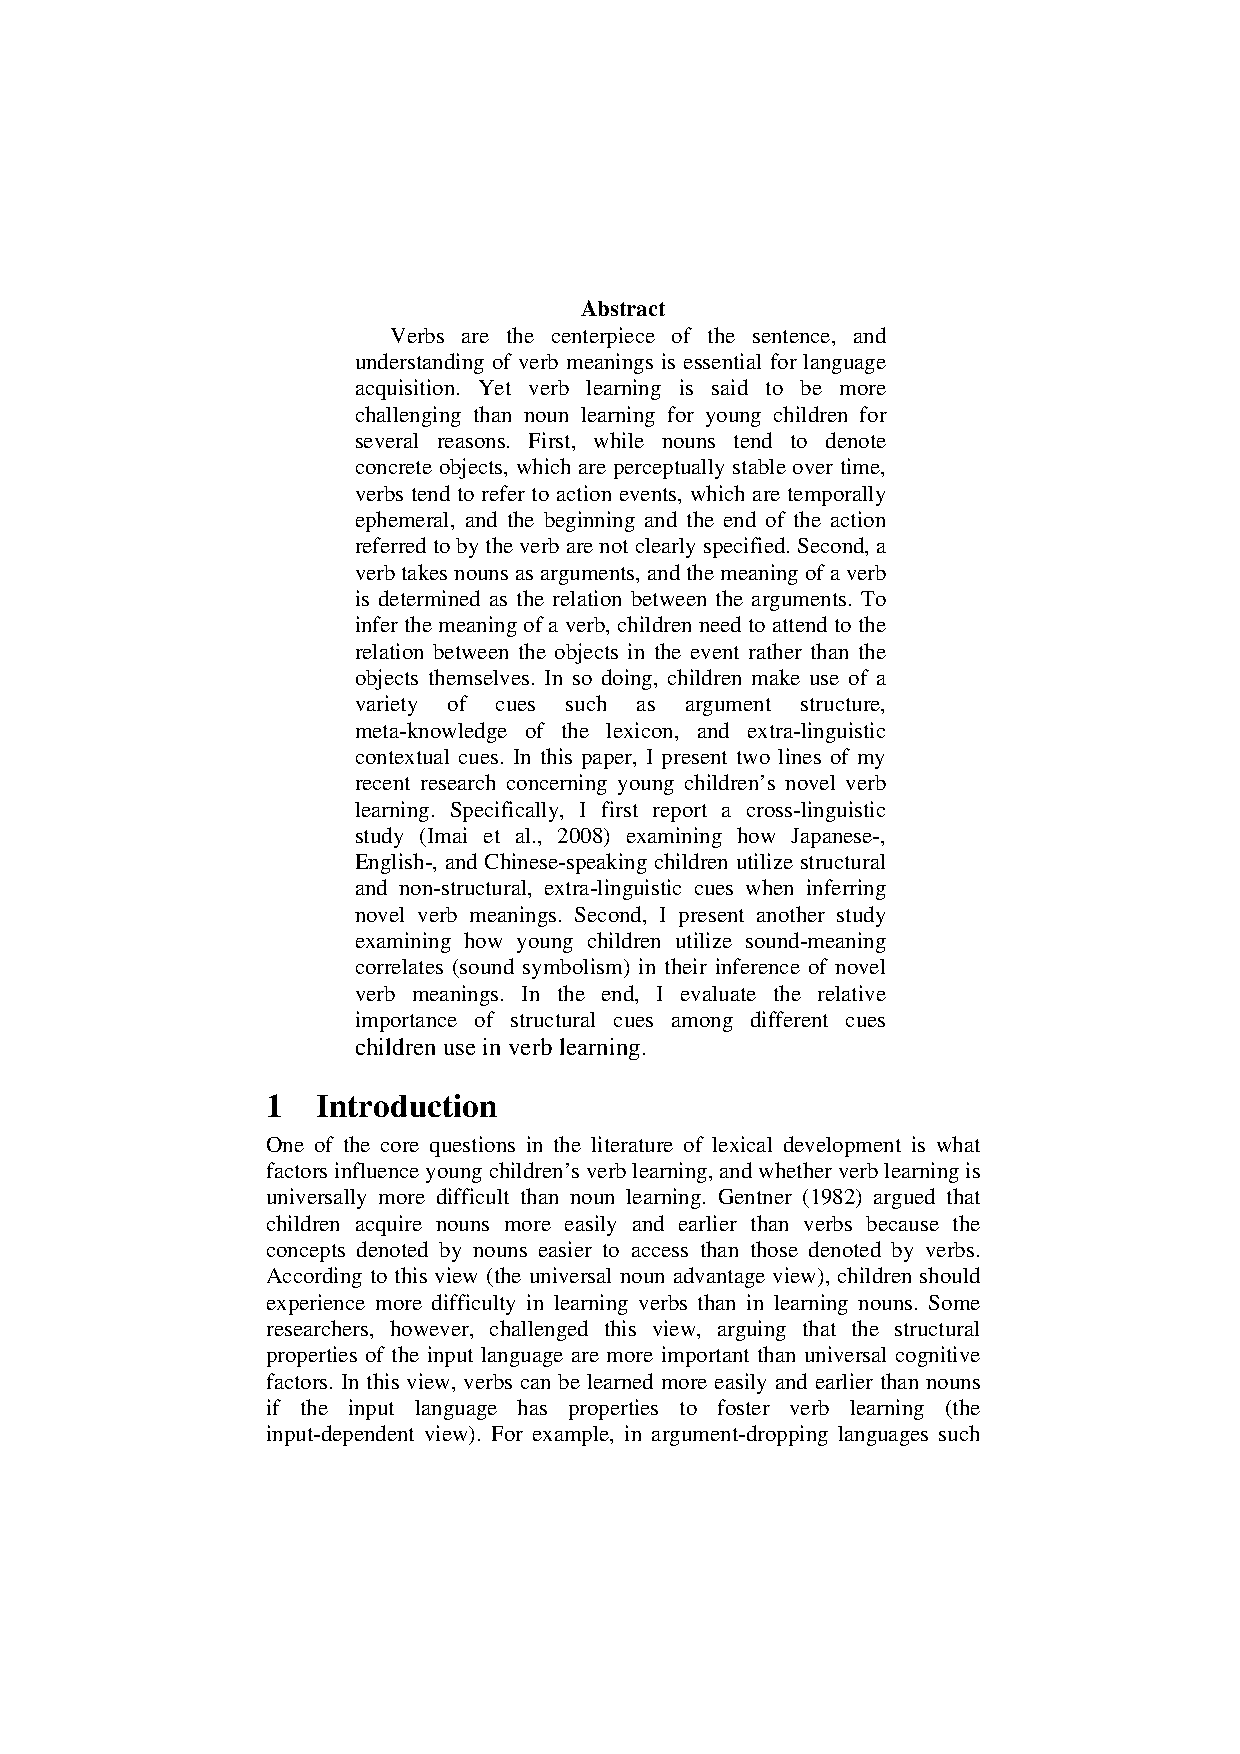
\includepdf[pages=-,pagecommand=\thispagestyle{plain}]{Includes/imai.pdf}
        \setcounter{page}{417}
        \phantomsection
        \addcontentsline{toc}{section}{Yusuke Kubota, Jungmee Lee: Reconsidering the Coordinate Structure Constraint in Japanese and Korean: Syntactic constraint or pragmatic principle?}
\thispagestyle{empty}

\begin{center}
  {\huge\bfseries Reconsidering the Coordinate Structure Constraint in Japanese and Korean: Syntactic constraint or pragmatic principle?\par}

  \bigskip

~\\
\begingroup
\setlength{\leftskip}{0pt plus 1fill}
\setlength{\rightskip}{0pt plus 1fill}
\setlength{\parindent}{0pt}
\setlength{\parfillskip}{0pt}
  \formatauthor{Yusuke Kubota}{\begin{tabular}{@{}c@{}}The Ohio State University\end{tabular}}
\formatauthor{Jungmee Lee}{\begin{tabular}{@{}c@{}}The Ohio State University\end{tabular}}

\par\endgroup

  \vspace*{8ex}

  Proceedings of the 15th International Conference on\par Head-Driven Phrase Structure Grammar

  \bigskip

  National Institute of Information and Communications Technology, Keihanna

  \medskip

  Stefan Müller (Editor)

  \medskip

  2008

  \medskip

  CSLI Publications

  \medskip

  pages 417--435

  \medskip

  \url{http://csli-publications.stanford.edu/HPSG/2008}
\end{center}
\vfill

\noindent



\vfill
\noindent
% APA Style
Kubota, Yusuke, \& Lee, Jungmee. 2008. Reconsidering the Coordinate Structure Constraint in Japanese and Korean: Syntactic constraint or pragmatic principle? In Müller, Stefan (Ed.), \emph{{Proceedings of the 15th International Conference on Head-Driven Phrase Structure Grammar, National Institute of Information and Communications Technology, Keihanna}}, 417--435. Stanford,
CA: CSLI Publications. \hfill\href{http://creativecommons.org/licenses/by/4.0/}{\includegraphics[height=.75em]{Includes/ccby.eps}}

\newpage
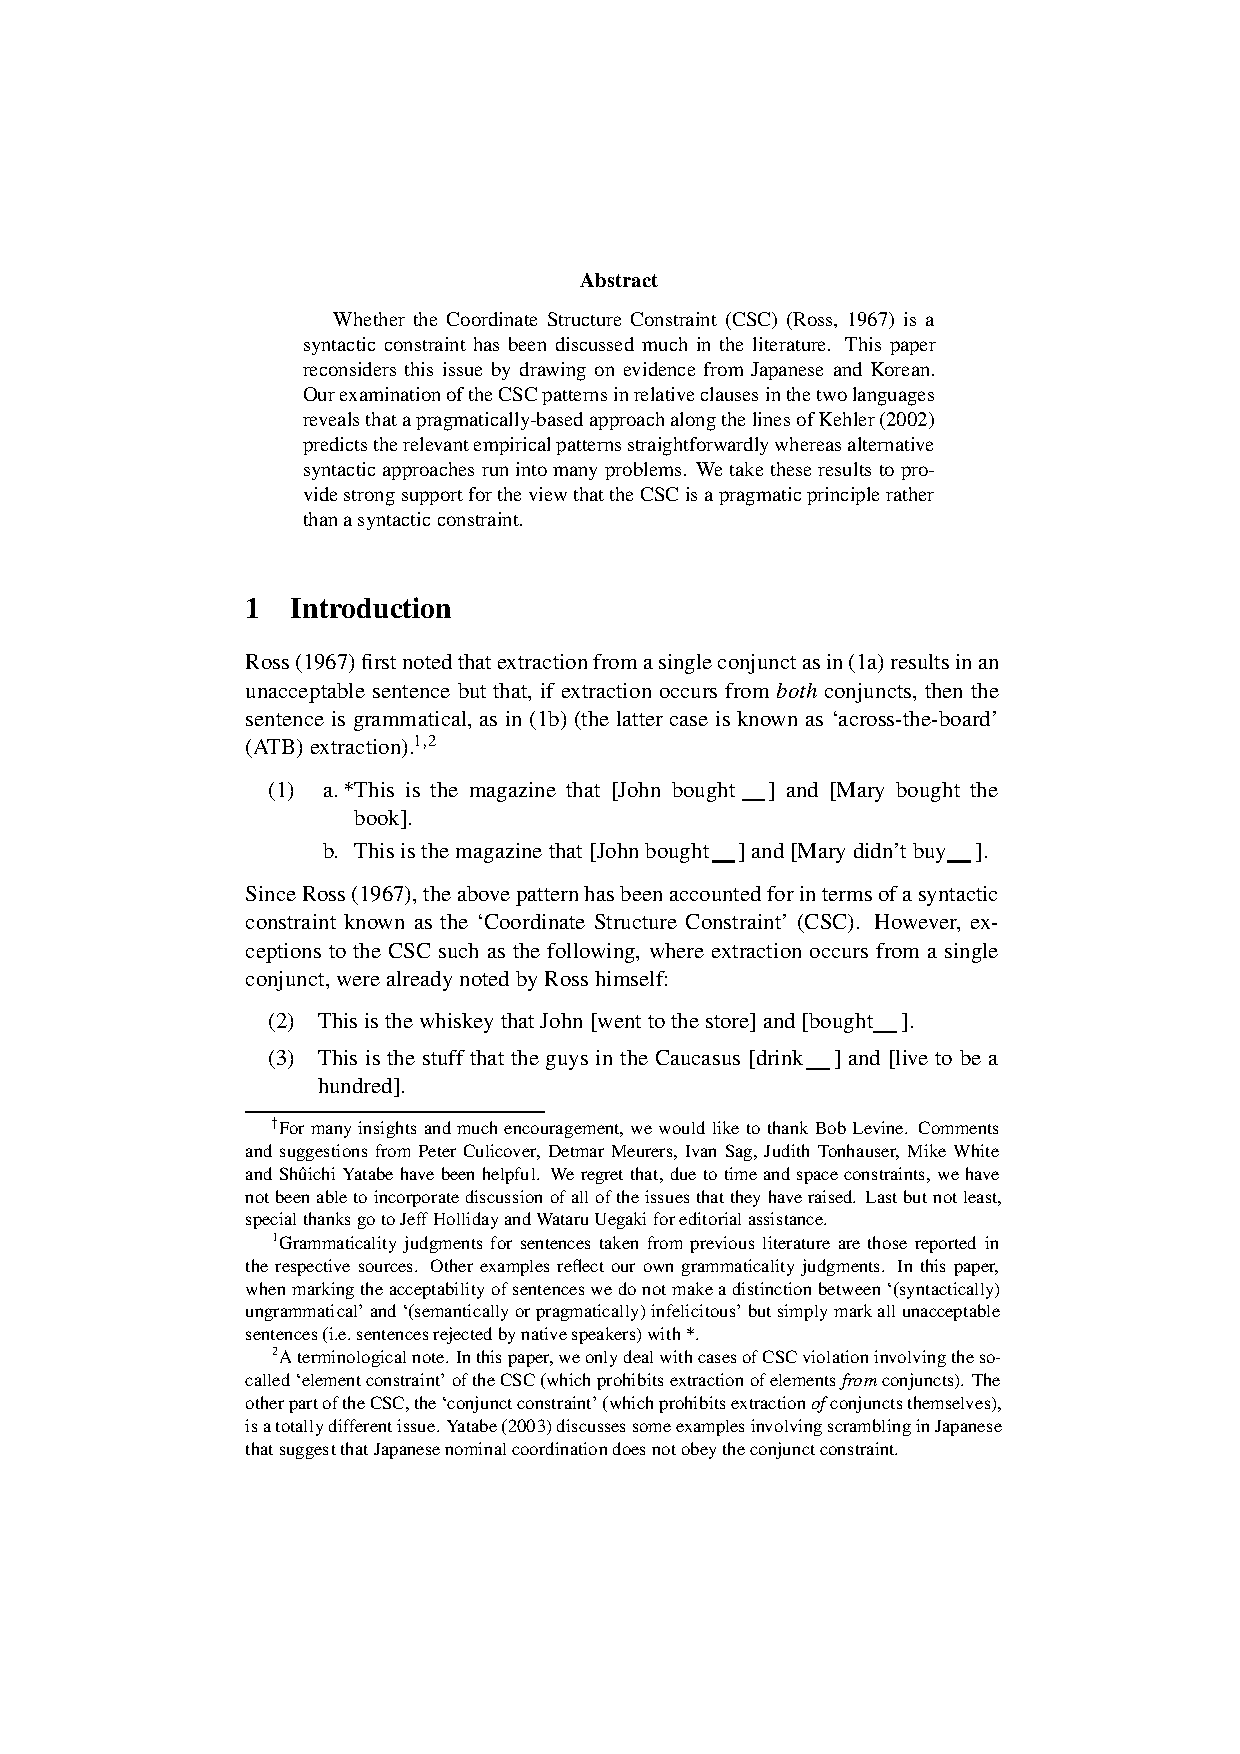
\includepdf[pages=-,pagecommand=\thispagestyle{plain}]{Includes/kubota-lee.pdf}
        \setcounter{page}{436}
        \phantomsection
        \addcontentsline{toc}{section}{Jean-Marie Marandin: The Exclamative Clause Type in French}
\thispagestyle{empty}

\begin{center}
  {\huge\bfseries The Exclamative Clause Type in French\par}

  \bigskip

~\\
\begingroup
\setlength{\leftskip}{0pt plus 1fill}
\setlength{\rightskip}{0pt plus 1fill}
\setlength{\parindent}{0pt}
\setlength{\parfillskip}{0pt}
  \formatauthor{Jean-Marie Marandin}{\begin{tabular}{@{}c@{}}CNRS, Université Paris 7\end{tabular}}

\par\endgroup

  \vspace*{8ex}

  Proceedings of the 15th International Conference on\par Head-Driven Phrase Structure Grammar

  \bigskip

  National Institute of Information and Communications Technology, Keihanna

  \medskip

  Stefan Müller (Editor)

  \medskip

  2008

  \medskip

  CSLI Publications

  \medskip

  pages 436--456

  \medskip

  \url{http://csli-publications.stanford.edu/HPSG/2008}
\end{center}
\vfill

\noindent



\vfill
\noindent
% APA Style
Marandin, Jean-Marie. 2008. The Exclamative Clause Type in French. In Müller, Stefan (Ed.), \emph{{Proceedings of the 15th International Conference on Head-Driven Phrase Structure Grammar, National Institute of Information and Communications Technology, Keihanna}}, 436--456. Stanford,
CA: CSLI Publications. \hfill\href{http://creativecommons.org/licenses/by/4.0/}{\includegraphics[height=.75em]{Includes/ccby.eps}}

\newpage
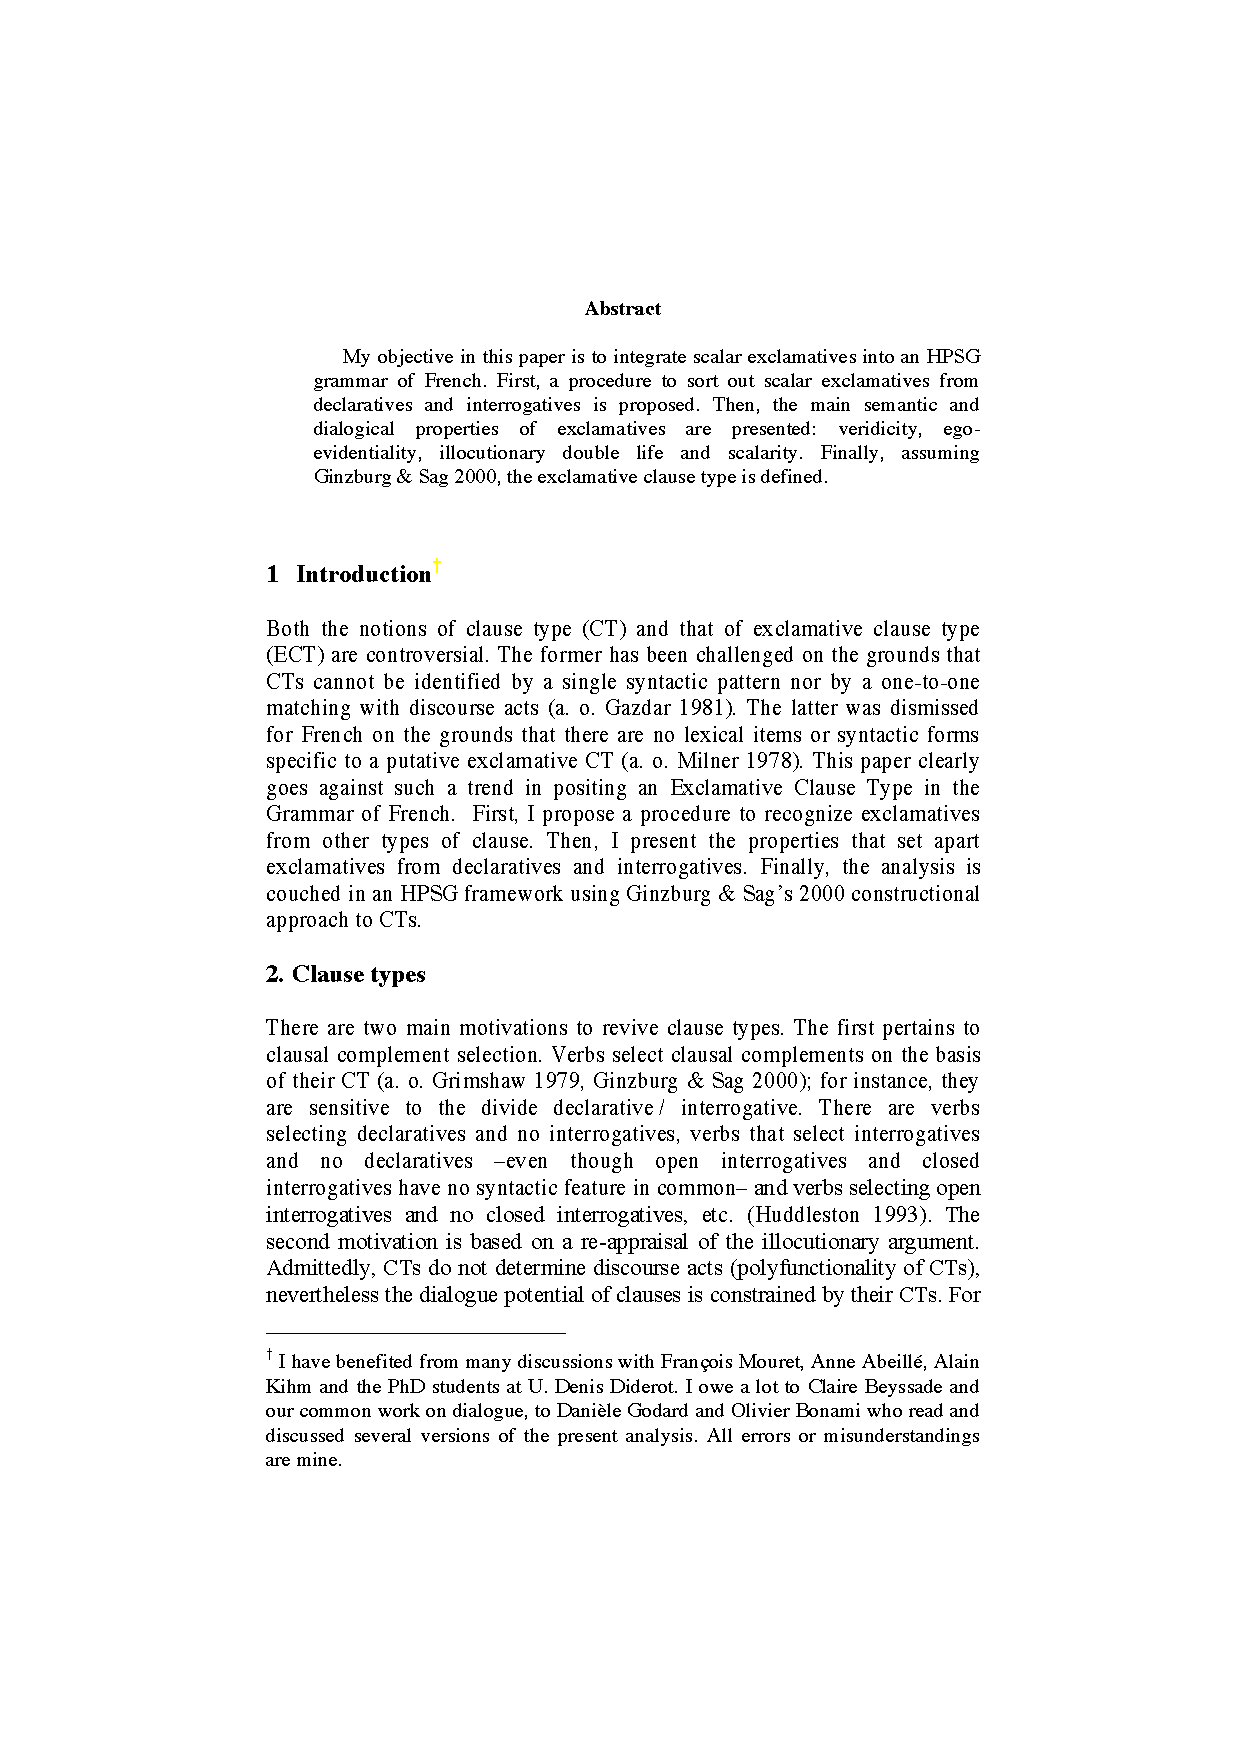
\includepdf[pages=-,pagecommand=\thispagestyle{plain}]{Includes/marandin.pdf}
\end{document}
